\documentclass[conf]{new-aiaa}
%\documentclass[journal]{new-aiaa} for journal papers
\usepackage[utf8]{inputenc}

\usepackage{graphicx}
\usepackage{amsmath}
\usepackage{commath}
\usepackage[version=4]{mhchem}
\usepackage{siunitx}
\usepackage{longtable,tabularx}
\usepackage{float}
\usepackage{listings}
\usepackage{pdfpages}
 \usepackage{booktabs}
\usepackage{color} %red, green, blue, yellow, cyan, magenta, black, white
\definecolor{mygreen}{RGB}{28,172,0} % color values Red, Green, Blue
\definecolor{mylilas}{RGB}{170,55,241}
\setlength\LTleft{0pt} 

\lstset{language=Matlab,%
	basicstyle=\footnotesize,
	breaklines=true,%
	morekeywords={matlab2tikz},
	keywordstyle=\color{blue},%
	morekeywords=[2]{1}, keywordstyle=[2]{\color{black}},
	identifierstyle=\color{black},%
	stringstyle=\color{mylilas},
	commentstyle=\color{mygreen},%
	showstringspaces=false,%without this there will be a symbol in the places where there is a space
	numbers=left,%
	numberstyle={\tiny \color{black}},% size of the numbers
	numbersep=9pt, % this defines how far the numbers are from the text
	emph=[1]{for,end,break},emphstyle=[1]\color{red}, %some words to emphasise
	%emph=[2]{word1,word2}, emphstyle=[2]{style},    
}

% ================================================================ % 
\title{ASE 389P.4 Methods of Orbit Determination \\ Term Project}

\author{Junette Hsin}
\affil{Masters Student, Aerospace Engineering and Engineering Mechanics, University of Texas, Austin, TX 78712}

\begin{document}

\maketitle

\begin{abstract}
	The theory and algorithms are derived and computer program to establish the trajectory of
	an Earth-orbiting satellite is developed. The assumptions for the study are:
	
	\begin{itemize}
		\item Three tracking stations taking apparent range and range-rate data are available for tracking the	satellite. Apparent quantities imply that the one-way light time between signal transmission and reception were modeled into the measurement (i.e. the effect is dealt with).
		\item The force model used to generate the truth is the EGM96 gravity field of degree and order 20,
		attitude-dependent solar radiation pressure, and atmospheric drag.
		\item The satellite is a box-wing shaped with one Sun-pointed solar panel with known component sizes, material properties, and orientation. The spacecraft -Z axis (in the spacecraft body reference frame) is always Nadir-pointed and has the antenna.
	\end{itemize}
	

\end{abstract}



% ================================================================ % 
\section*{Problem 1 and 2}

 % \subsubsection*{Statement} 
\begin{center}
\fbox{PREFIT and POSTFIT residuals for all data and all sensors.} \\
\end{center}

\begin{figure}[H]
	\centering
	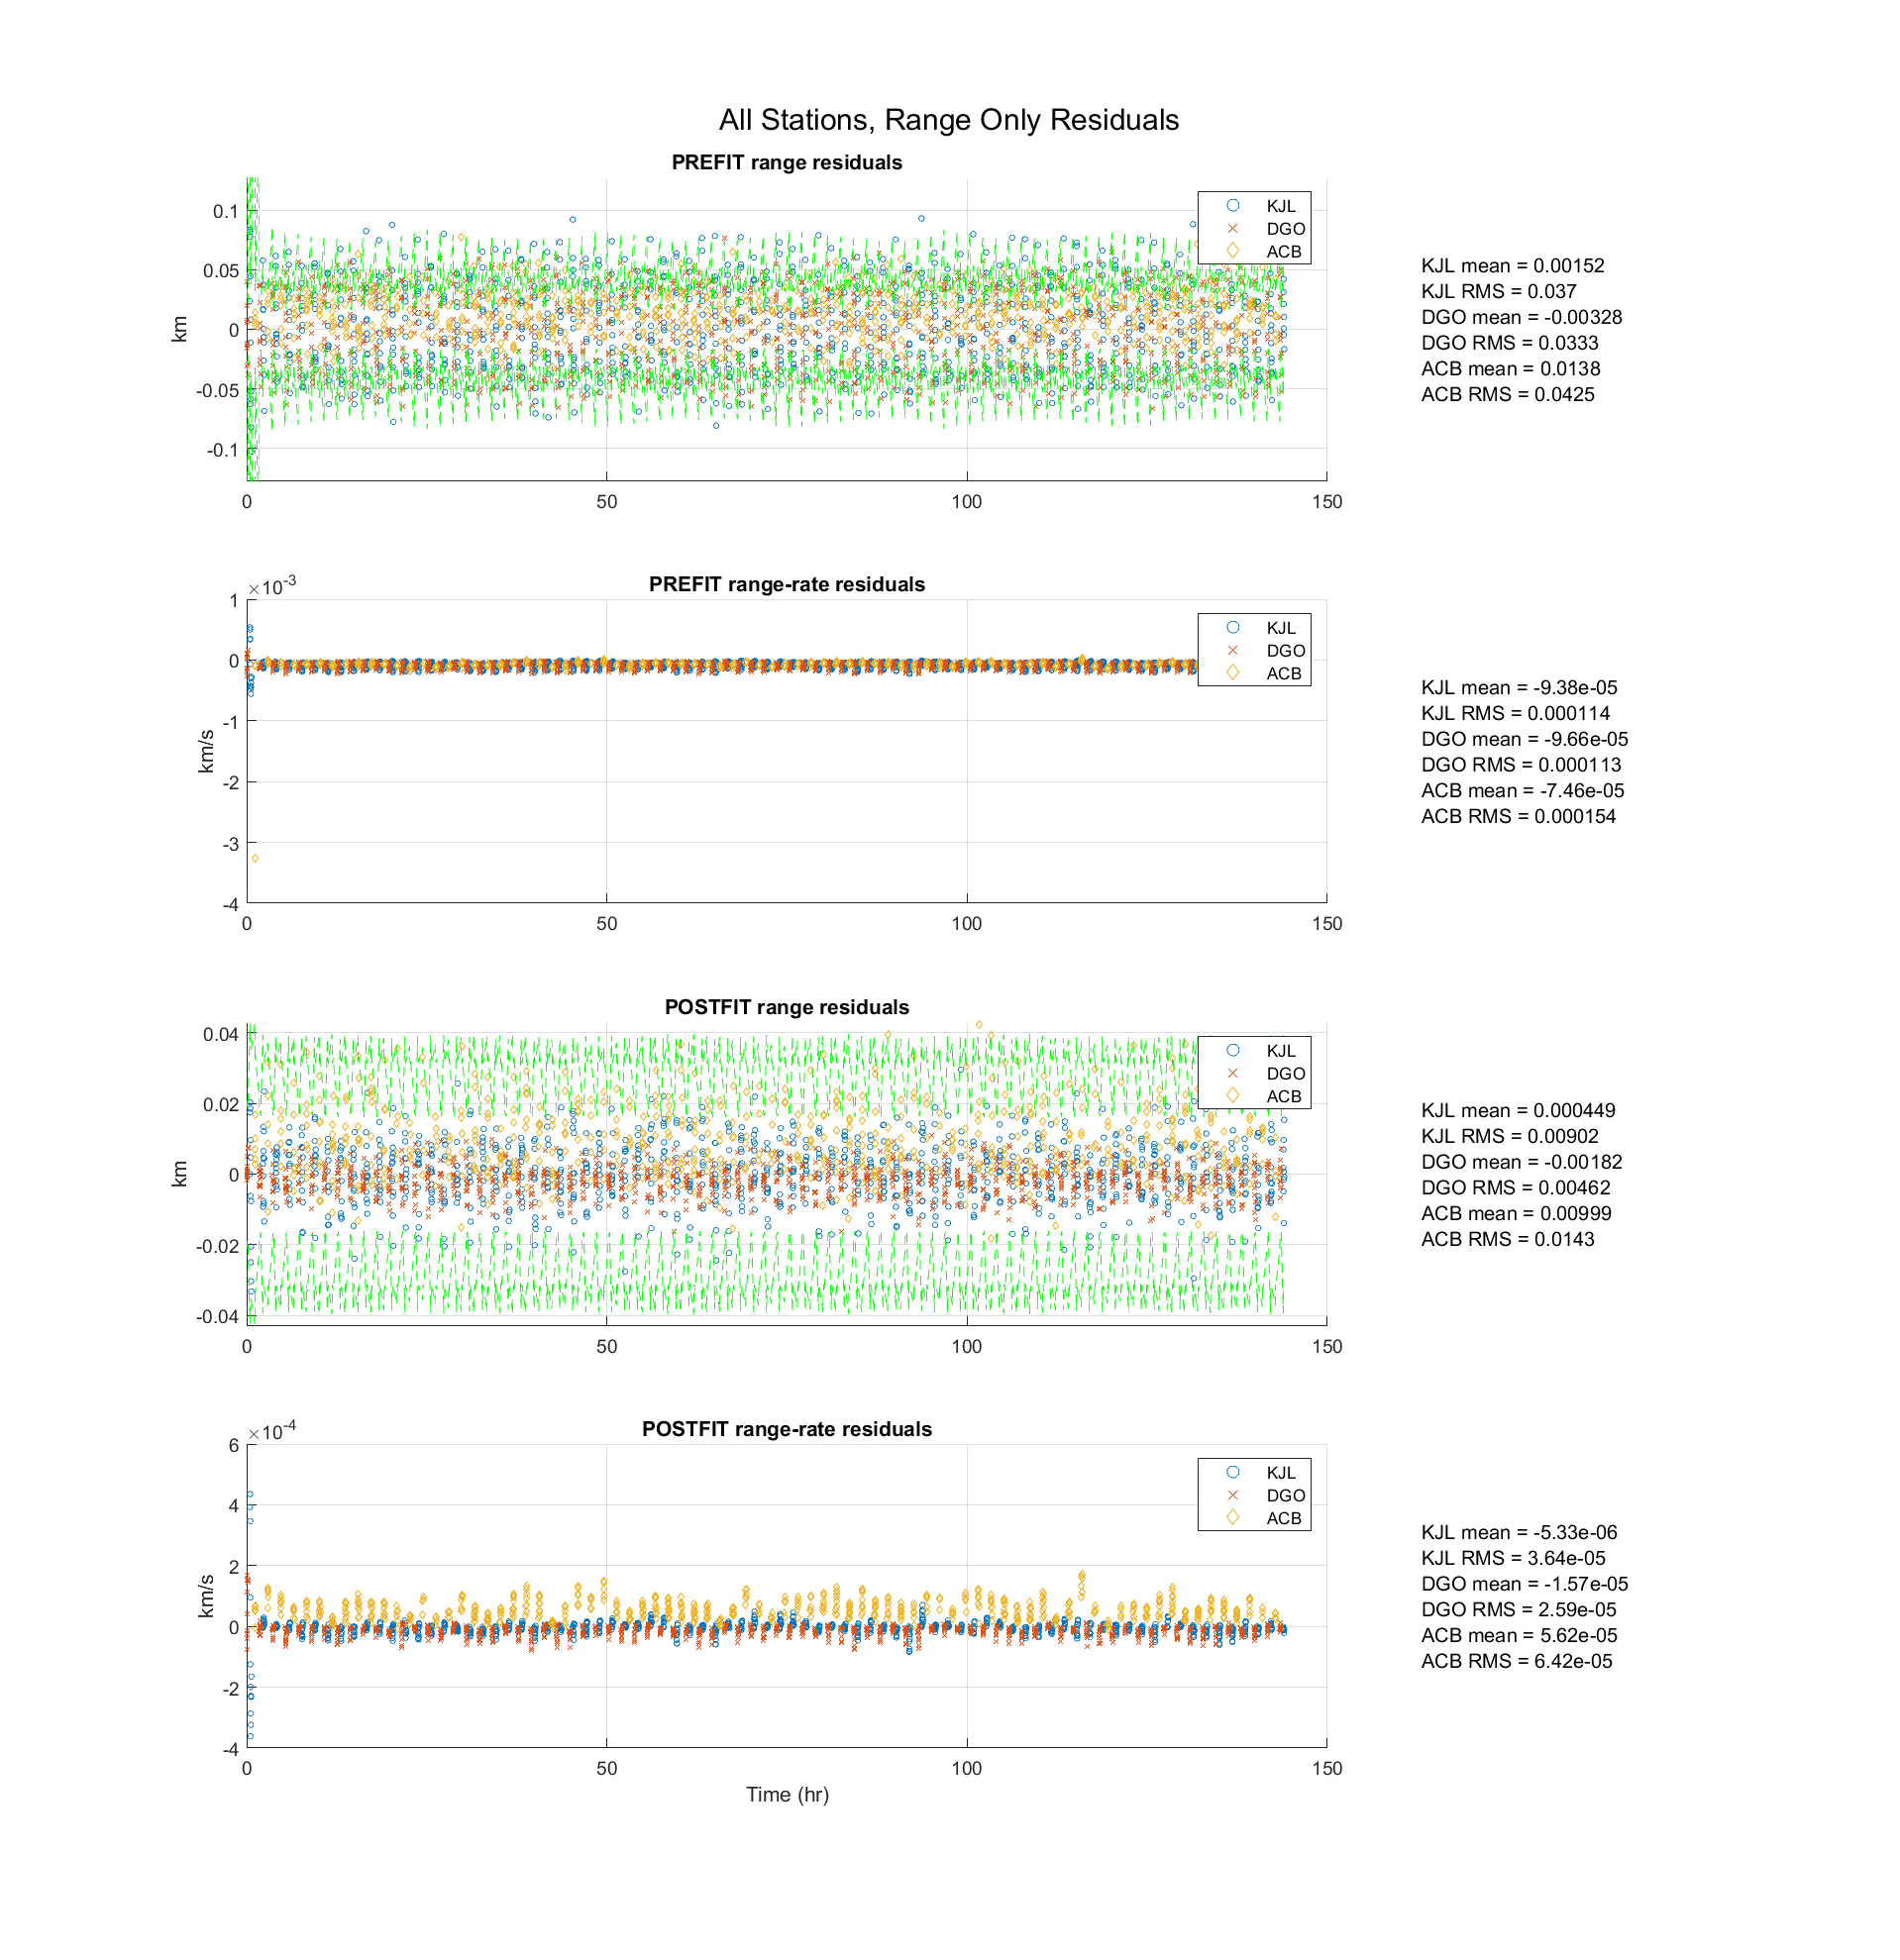
\includegraphics[width=\textwidth]{caseA_res.png}
	\caption{Case A: Range Only Prefit and Postfit Residuals}
\end{figure}

\begin{figure}[H]
\centering
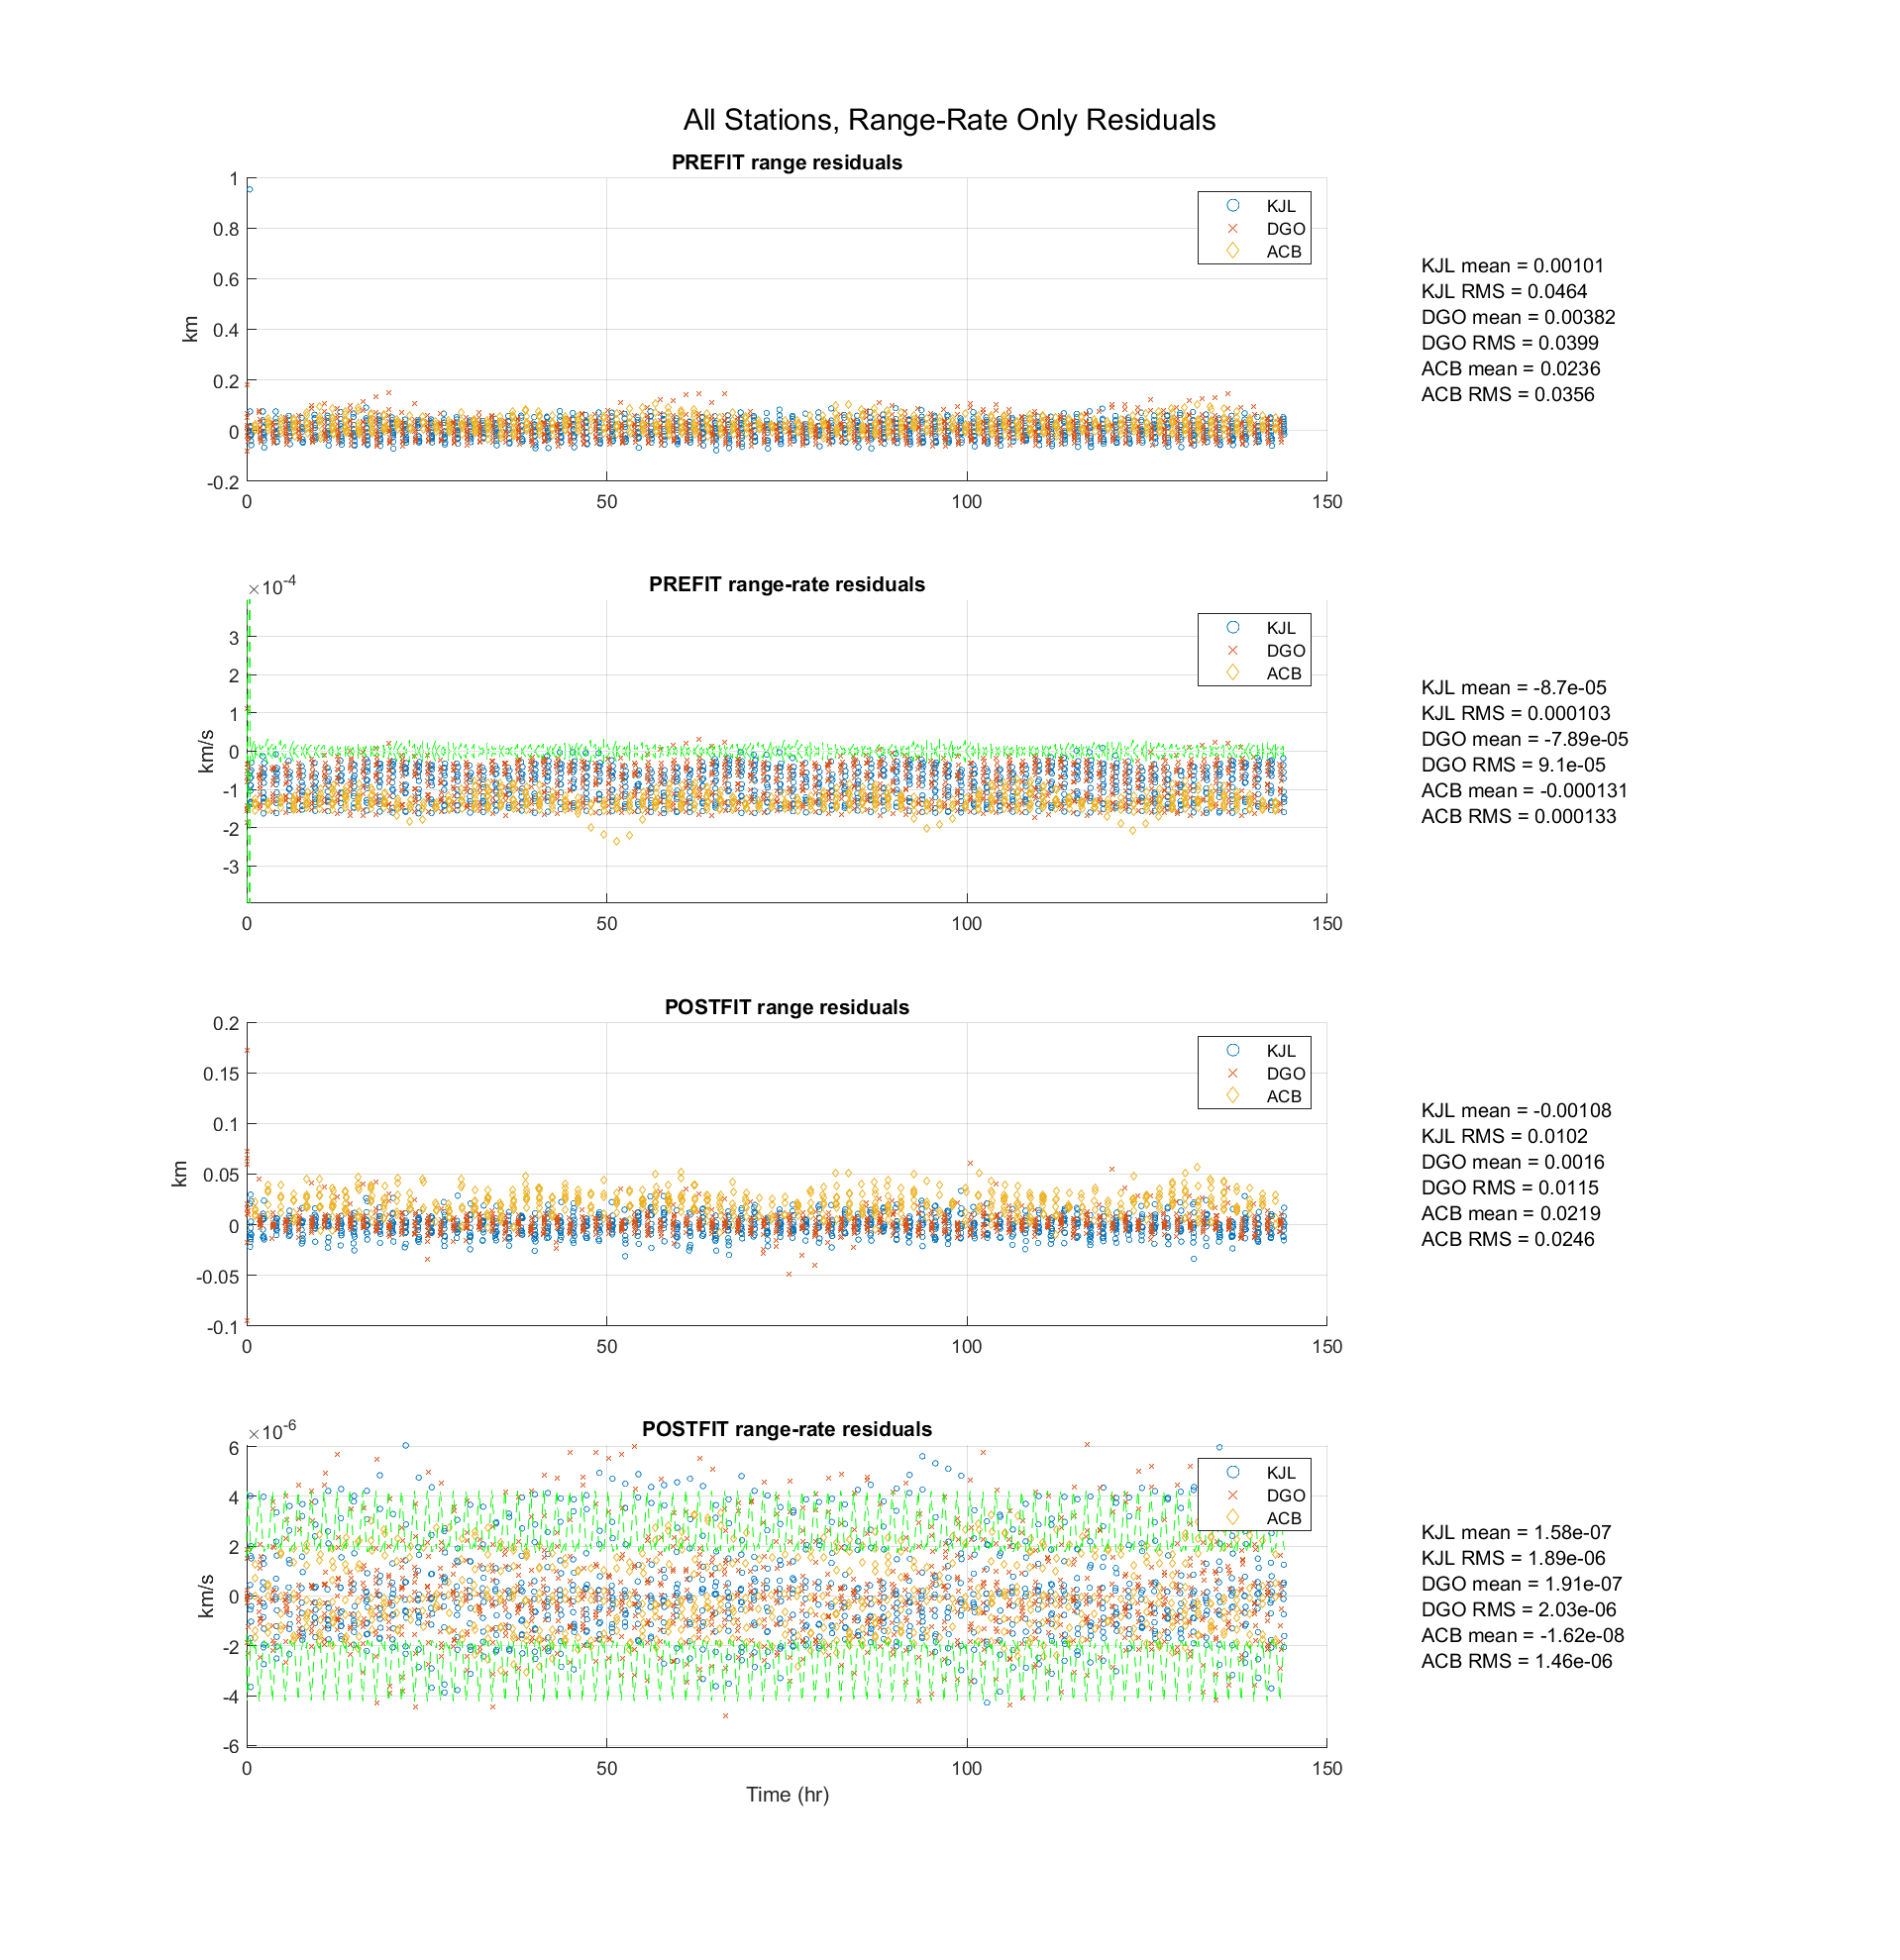
\includegraphics[width=\textwidth]{caseB_res.png}
\caption{Case B: Range-Rate Only Prefit and Postfit Residuals}
\end{figure}

\begin{figure}[H]
\centering
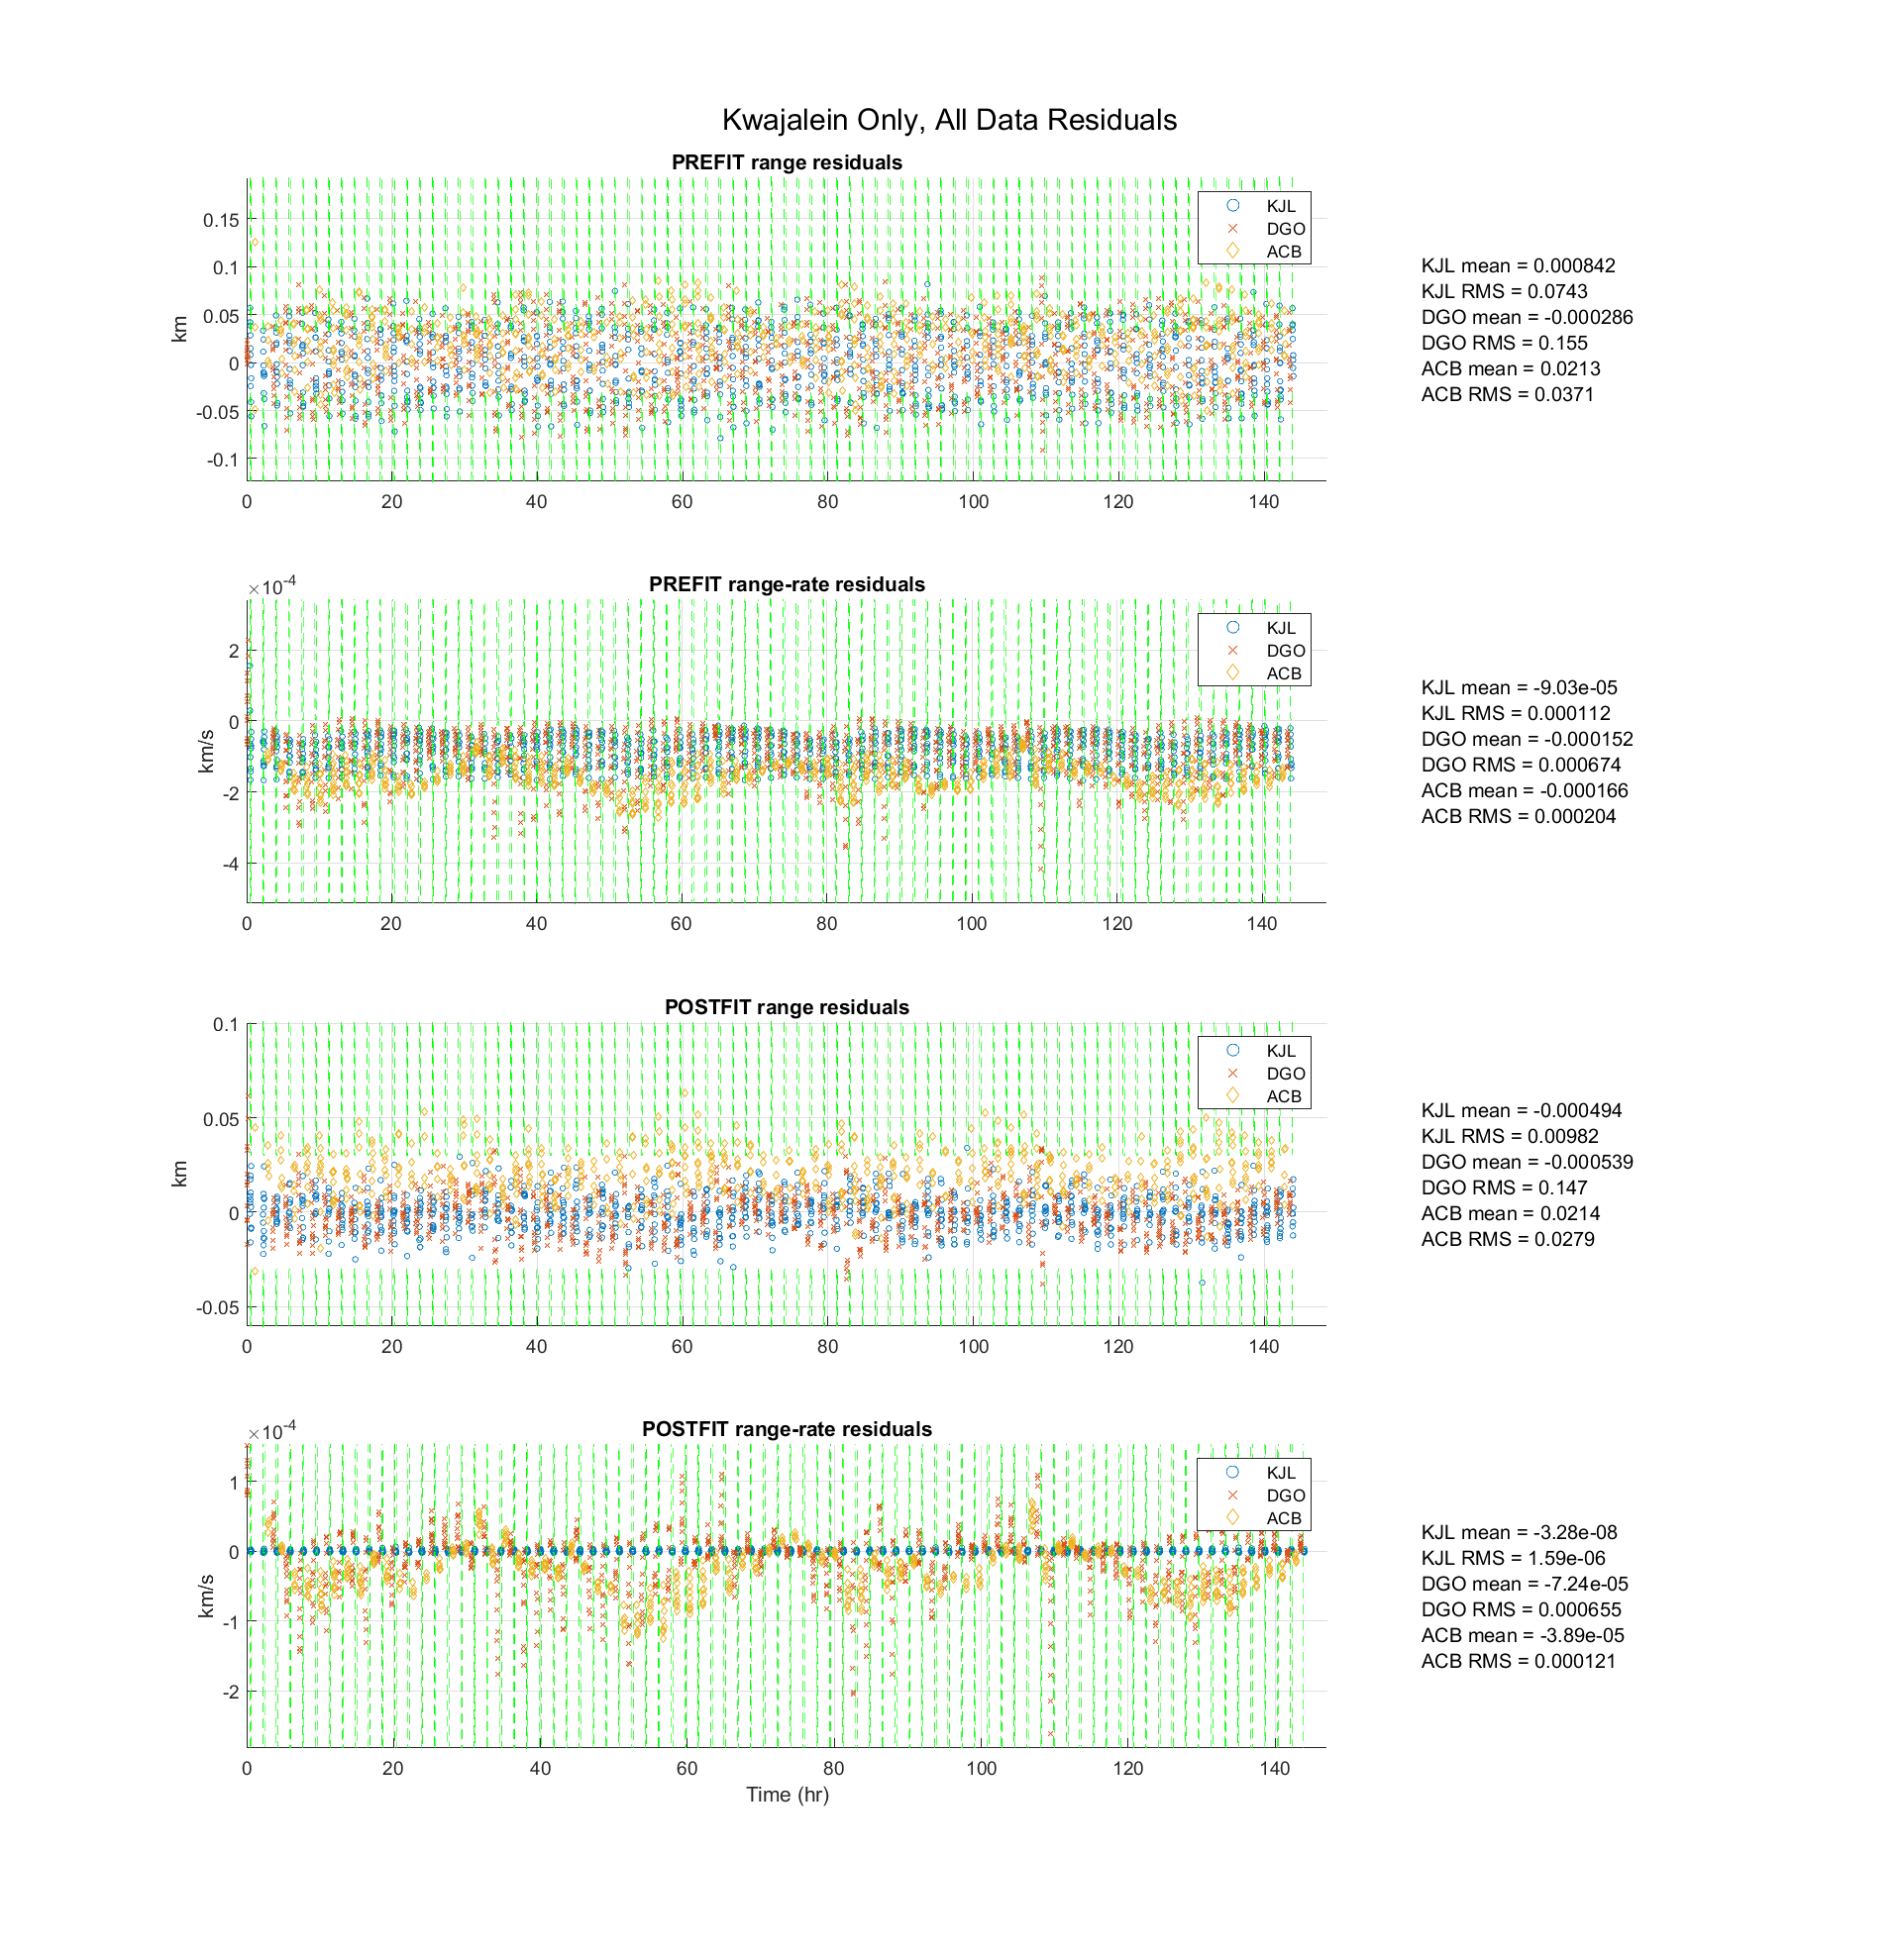
\includegraphics[width=\textwidth]{caseC_res.png}
\caption{Case C: Kwajalein Only Prefit and Postfit Residuals}
\end{figure}

\begin{figure}[H]
\centering
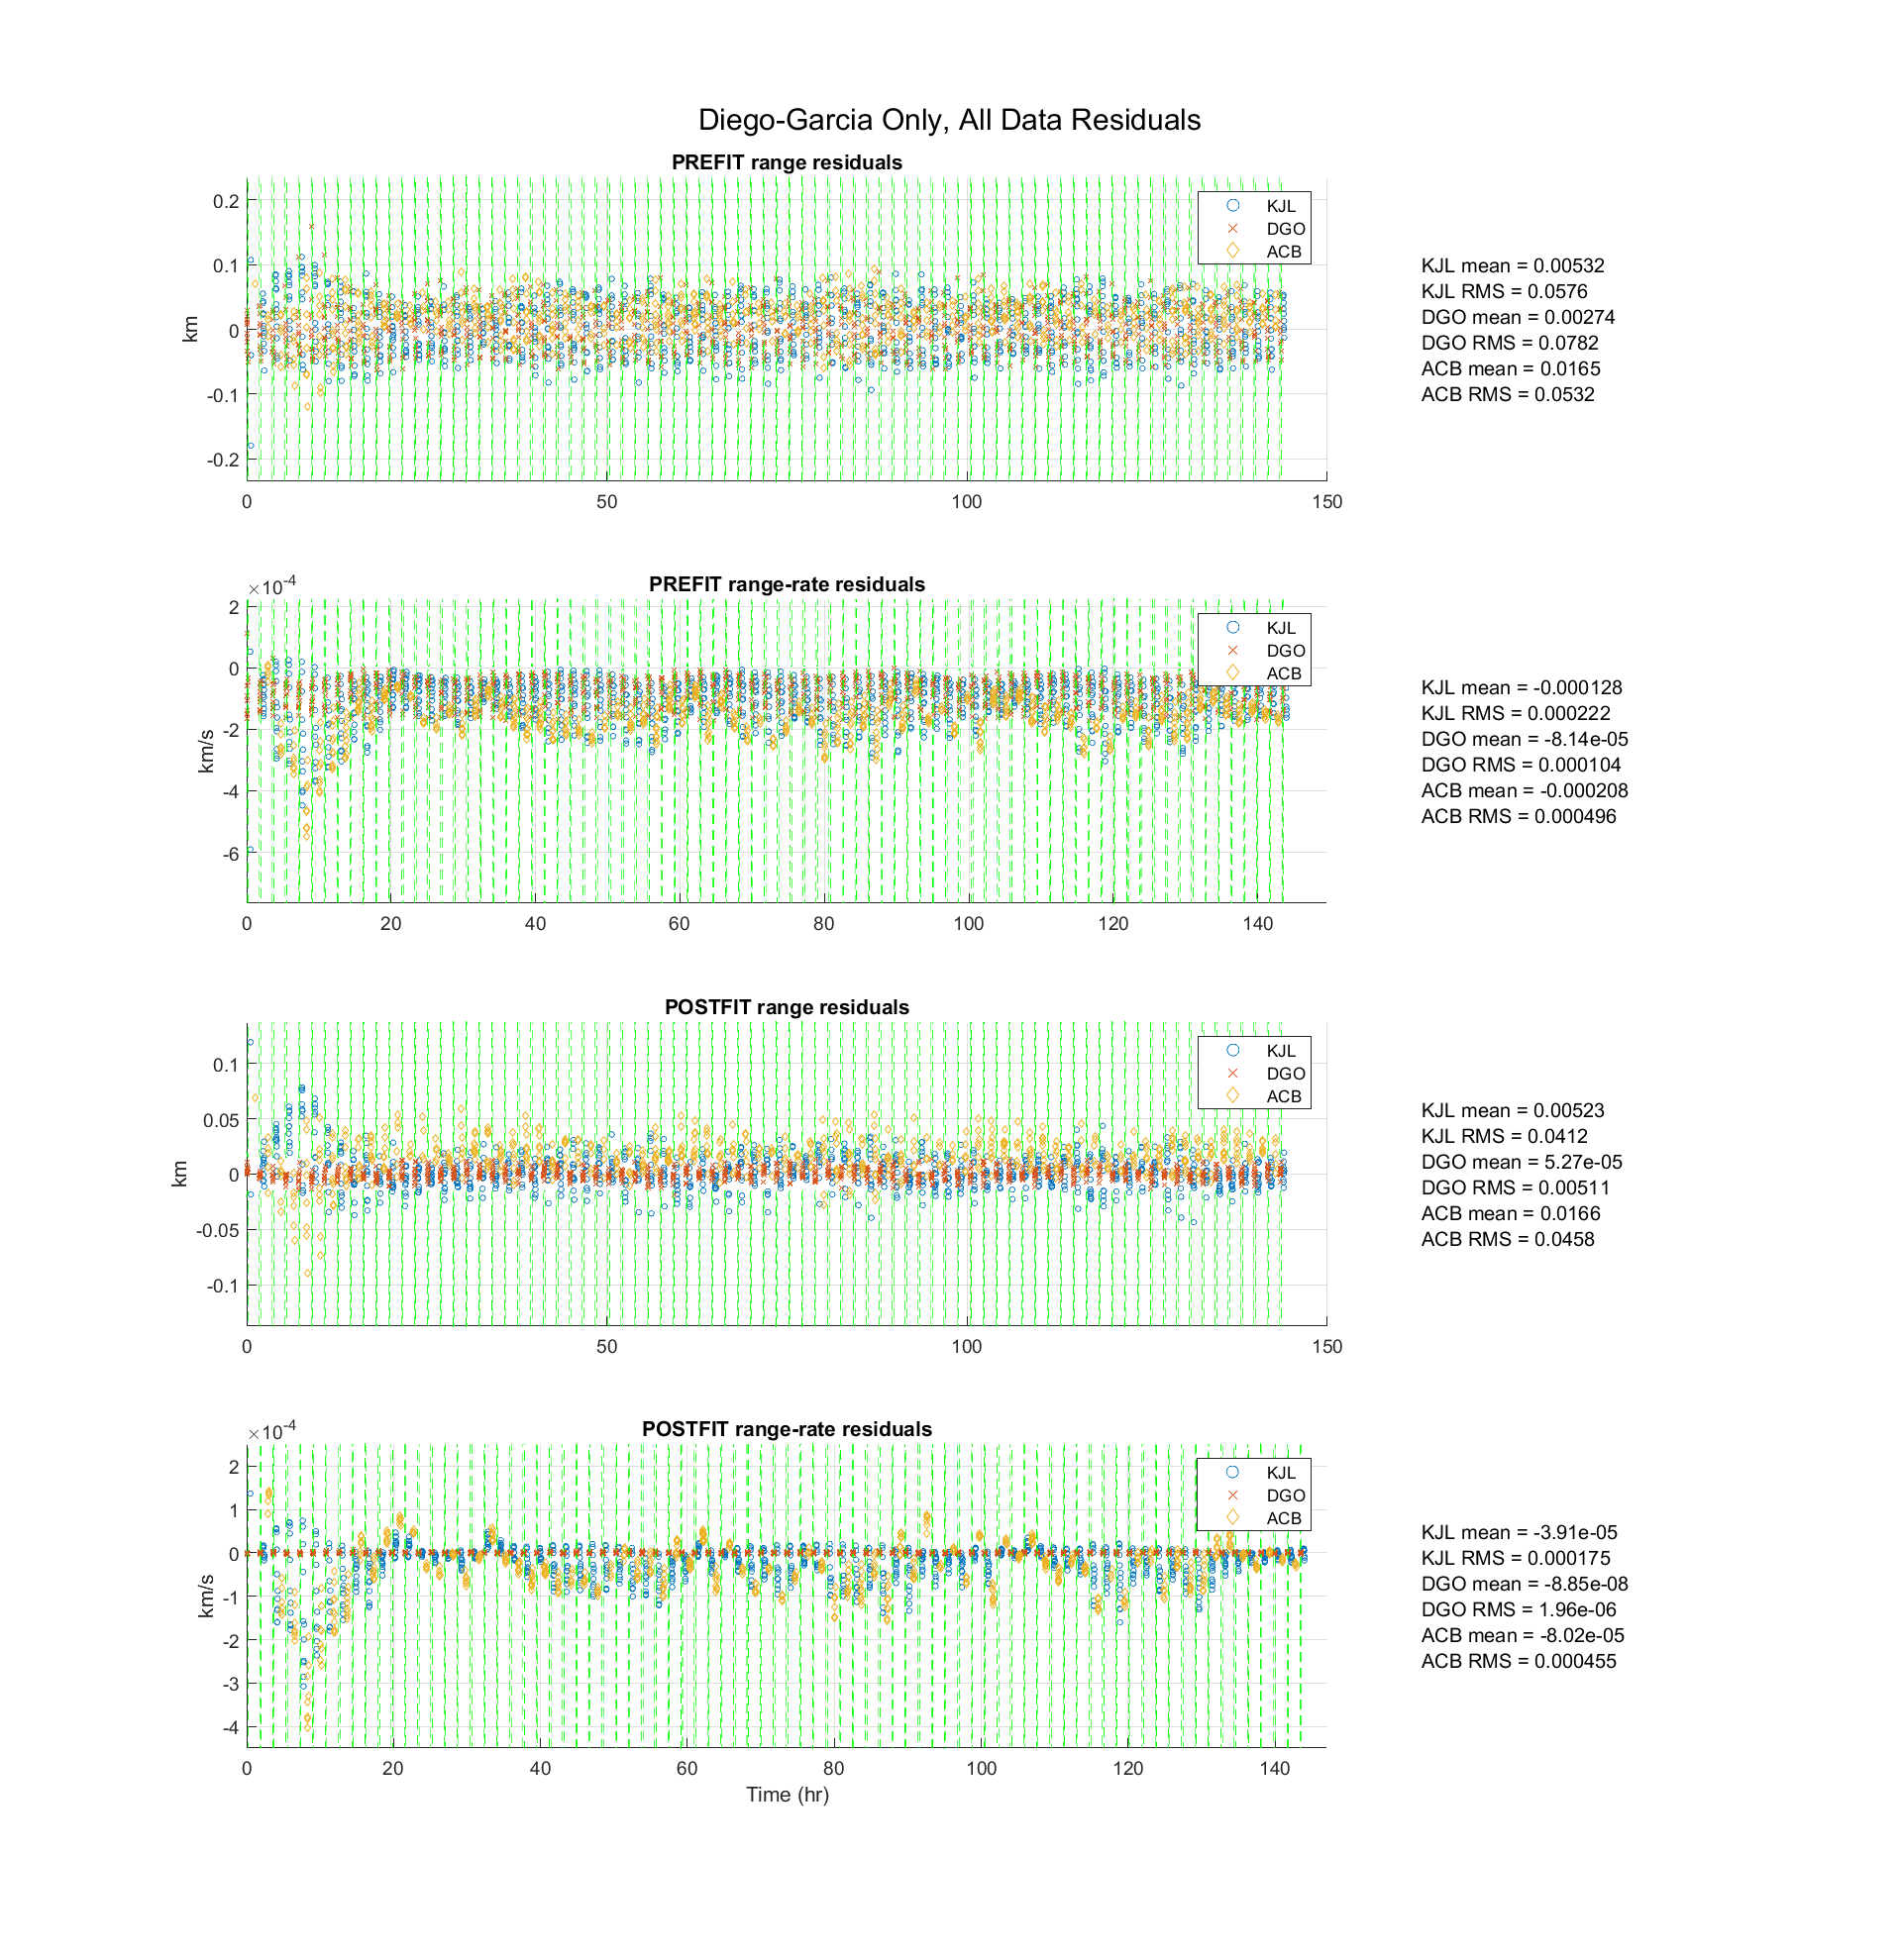
\includegraphics[width=\textwidth]{caseD_res.png}
\caption{Case D: Diego Garcia Only Prefit and Postfit Residuals}
\end{figure}

\begin{figure}[H]
\centering
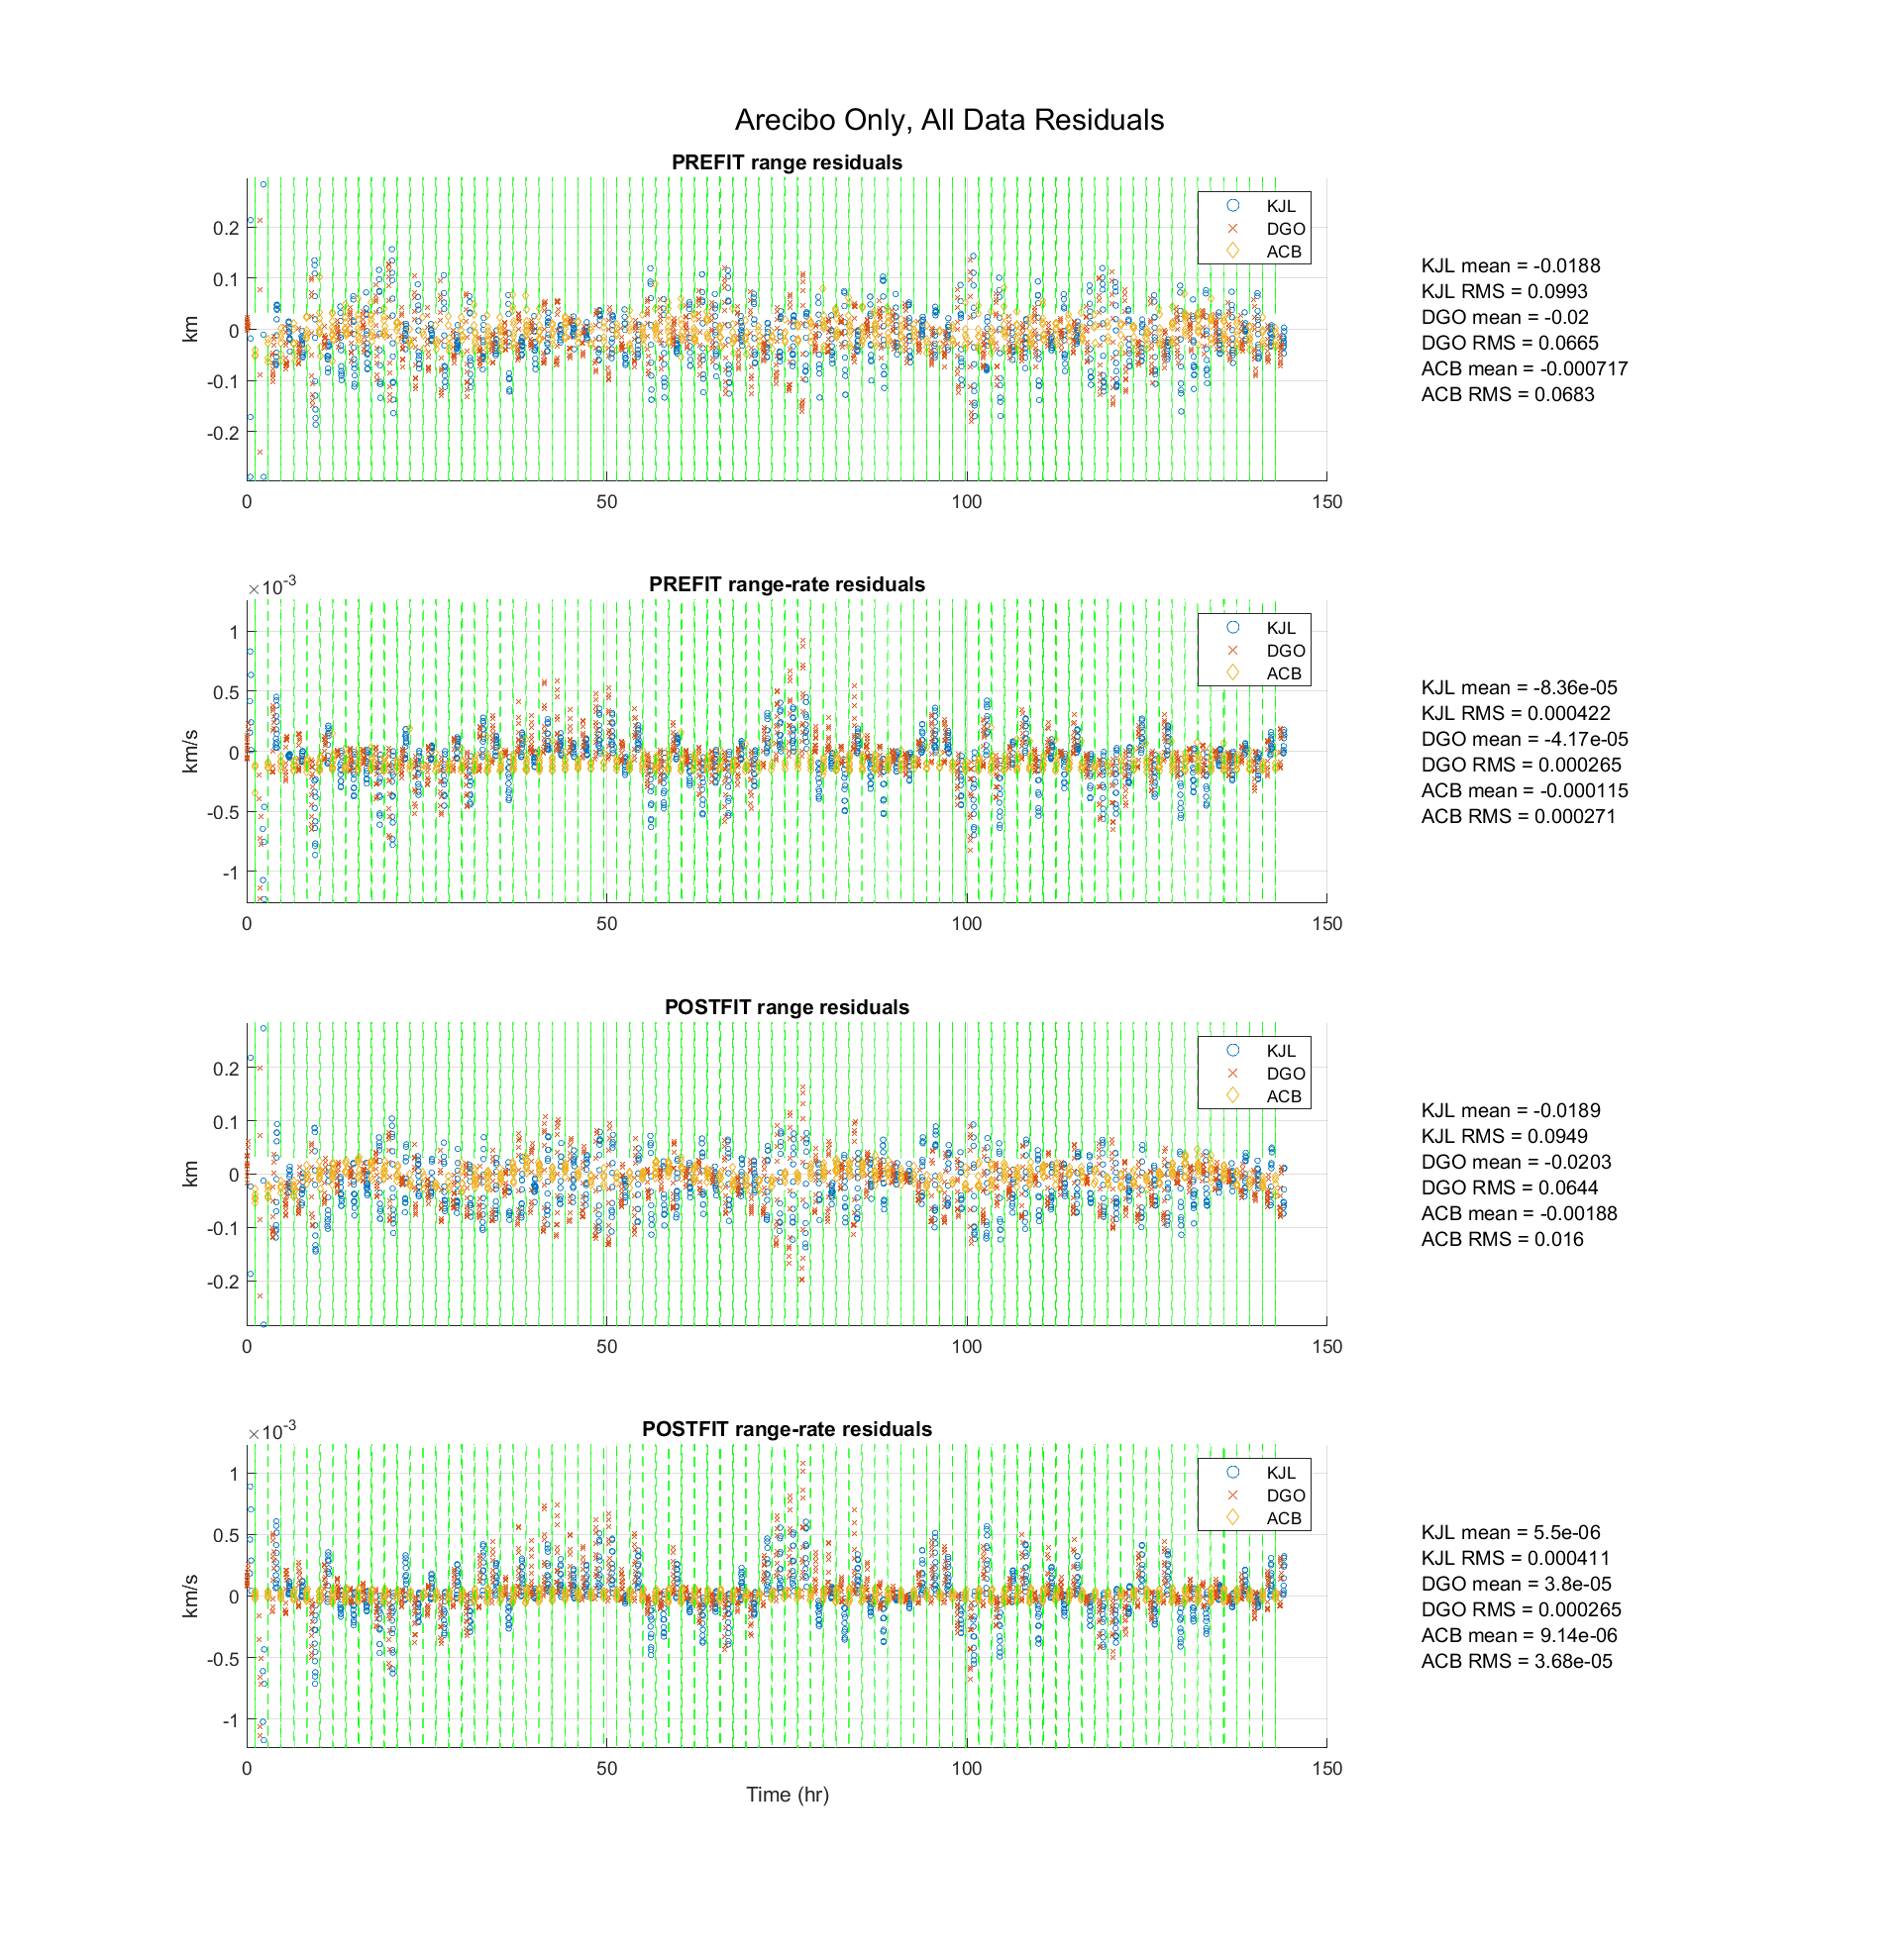
\includegraphics[width=\textwidth]{caseE_res.png}
\caption{Case E: Arecibo Only Prefit and Postfit Residuals}
\end{figure}

\begin{figure}[H]
\centering
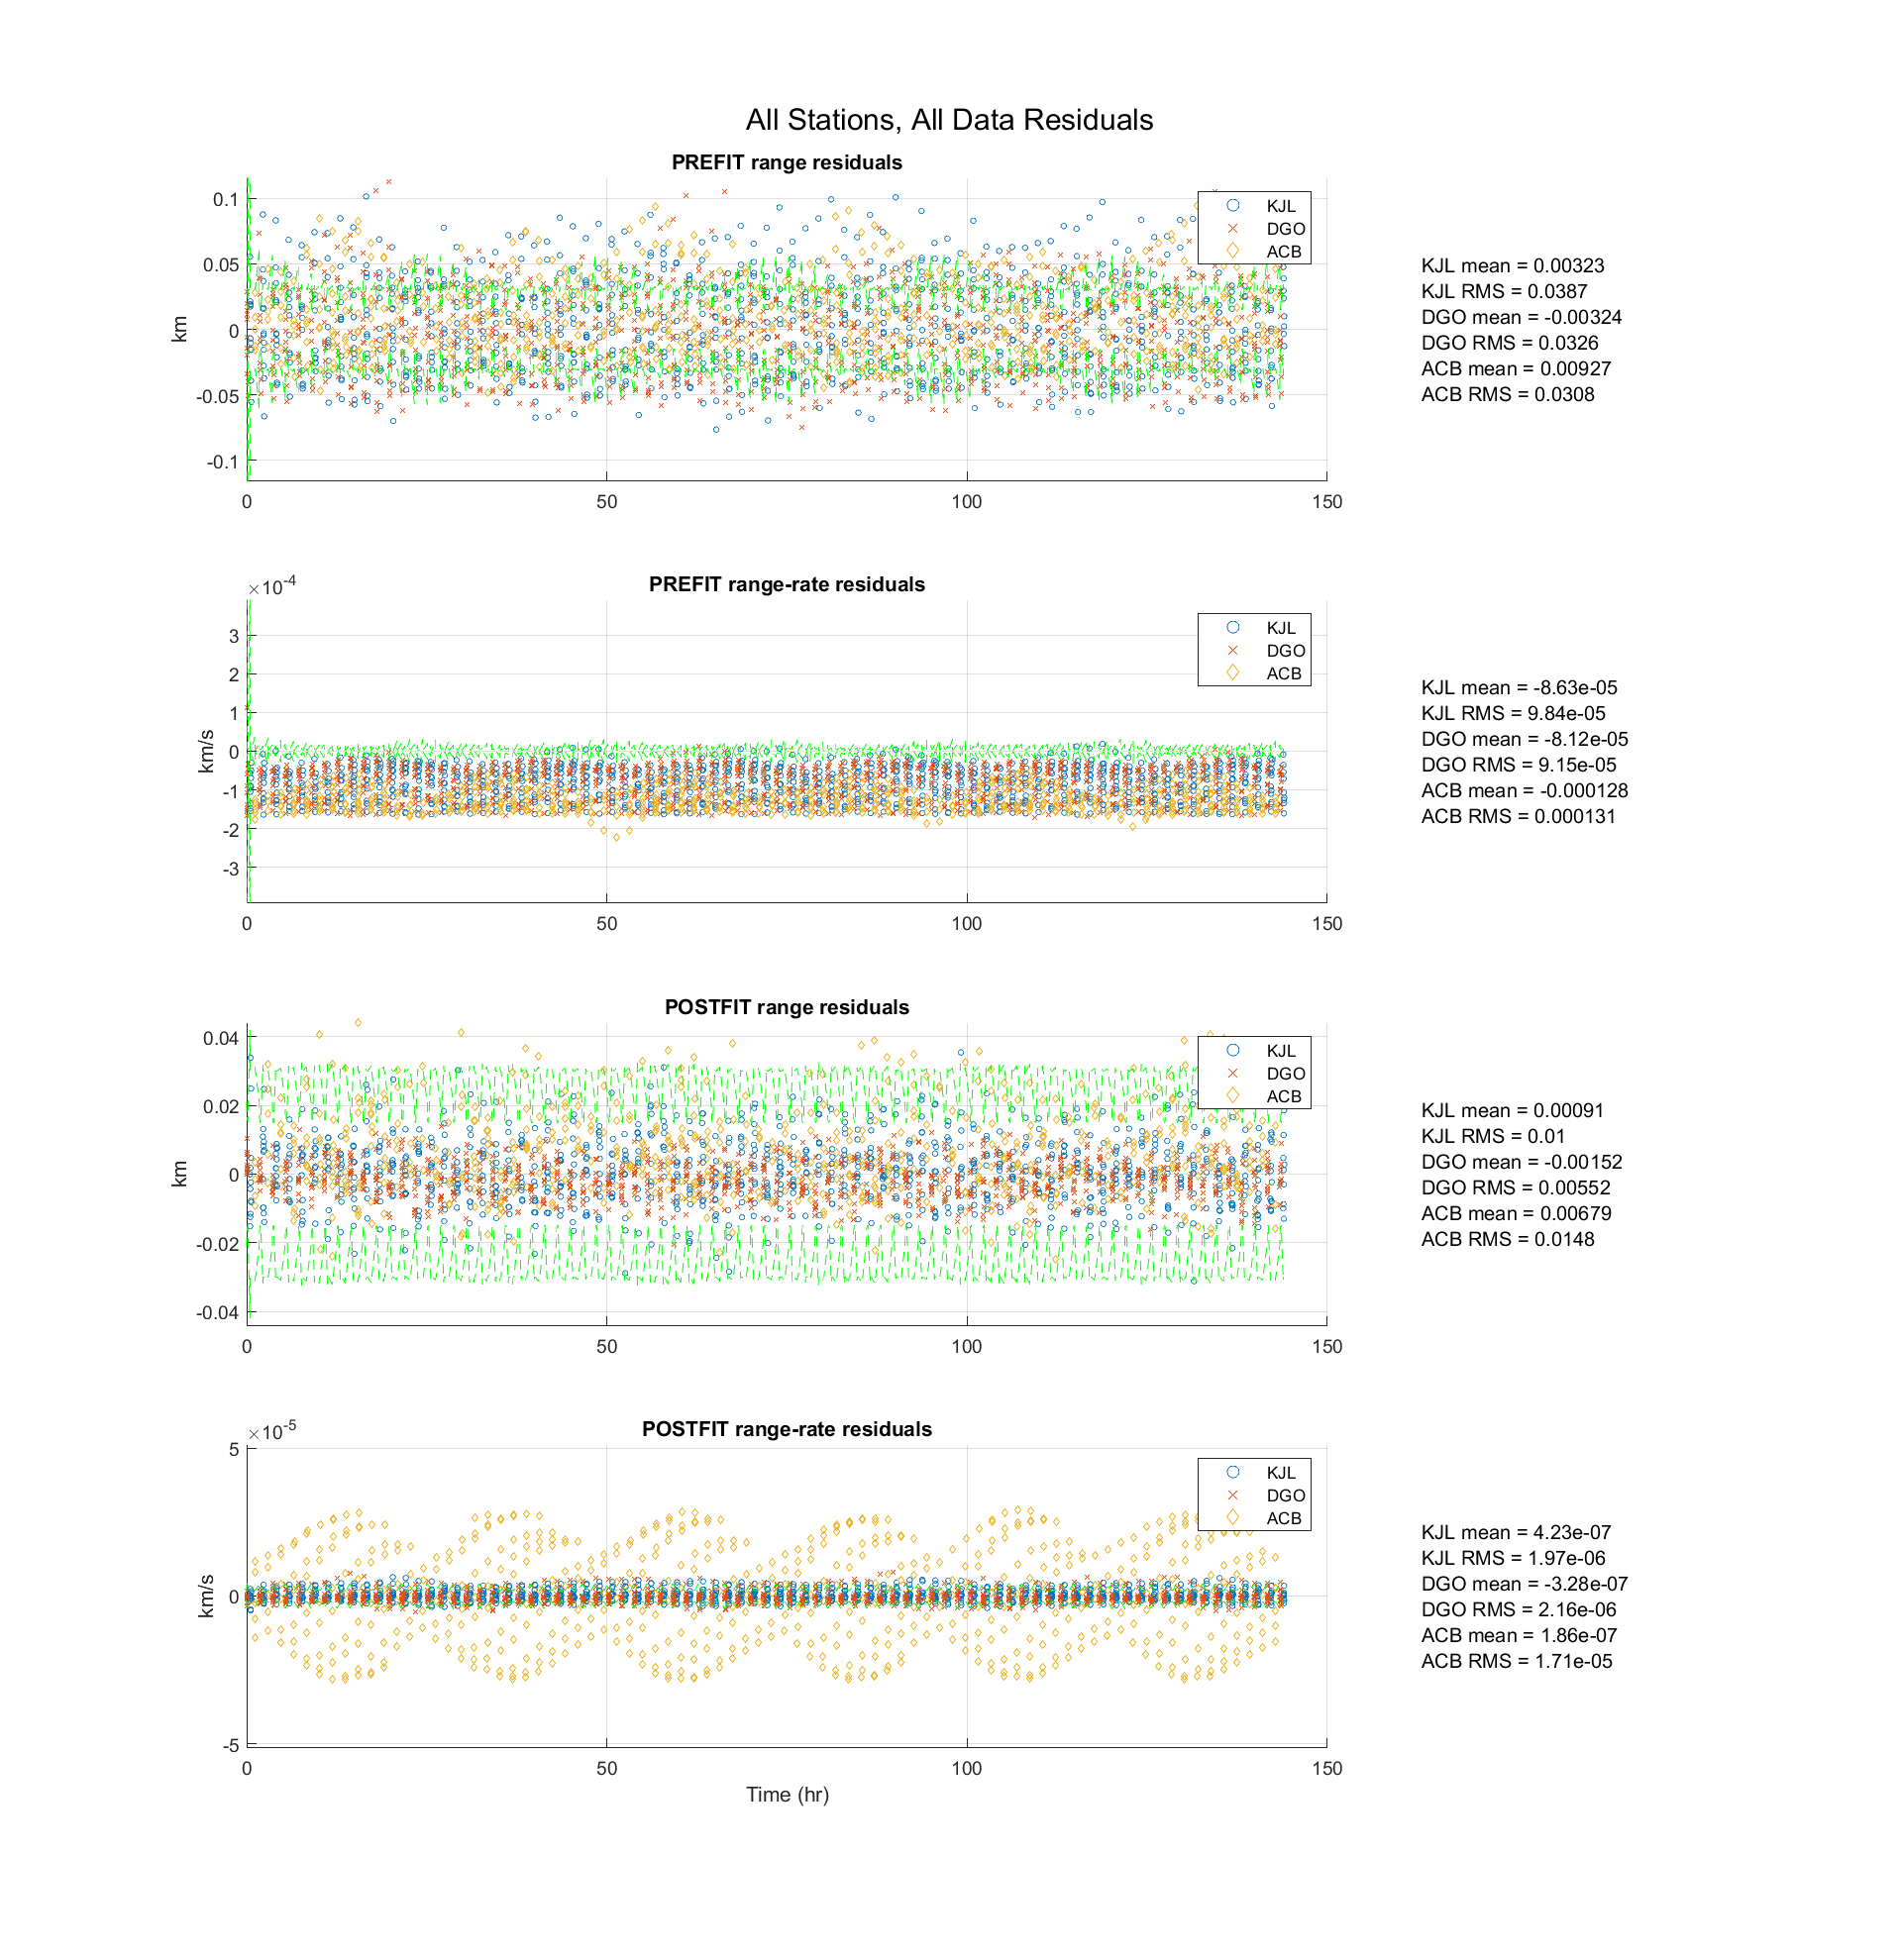
\includegraphics[width=\textwidth]{caseF_res.png}
\caption{Case F: Long-Arc Only Prefit and Postfit Residuals}
\end{figure}

\begin{figure}[H]
\centering
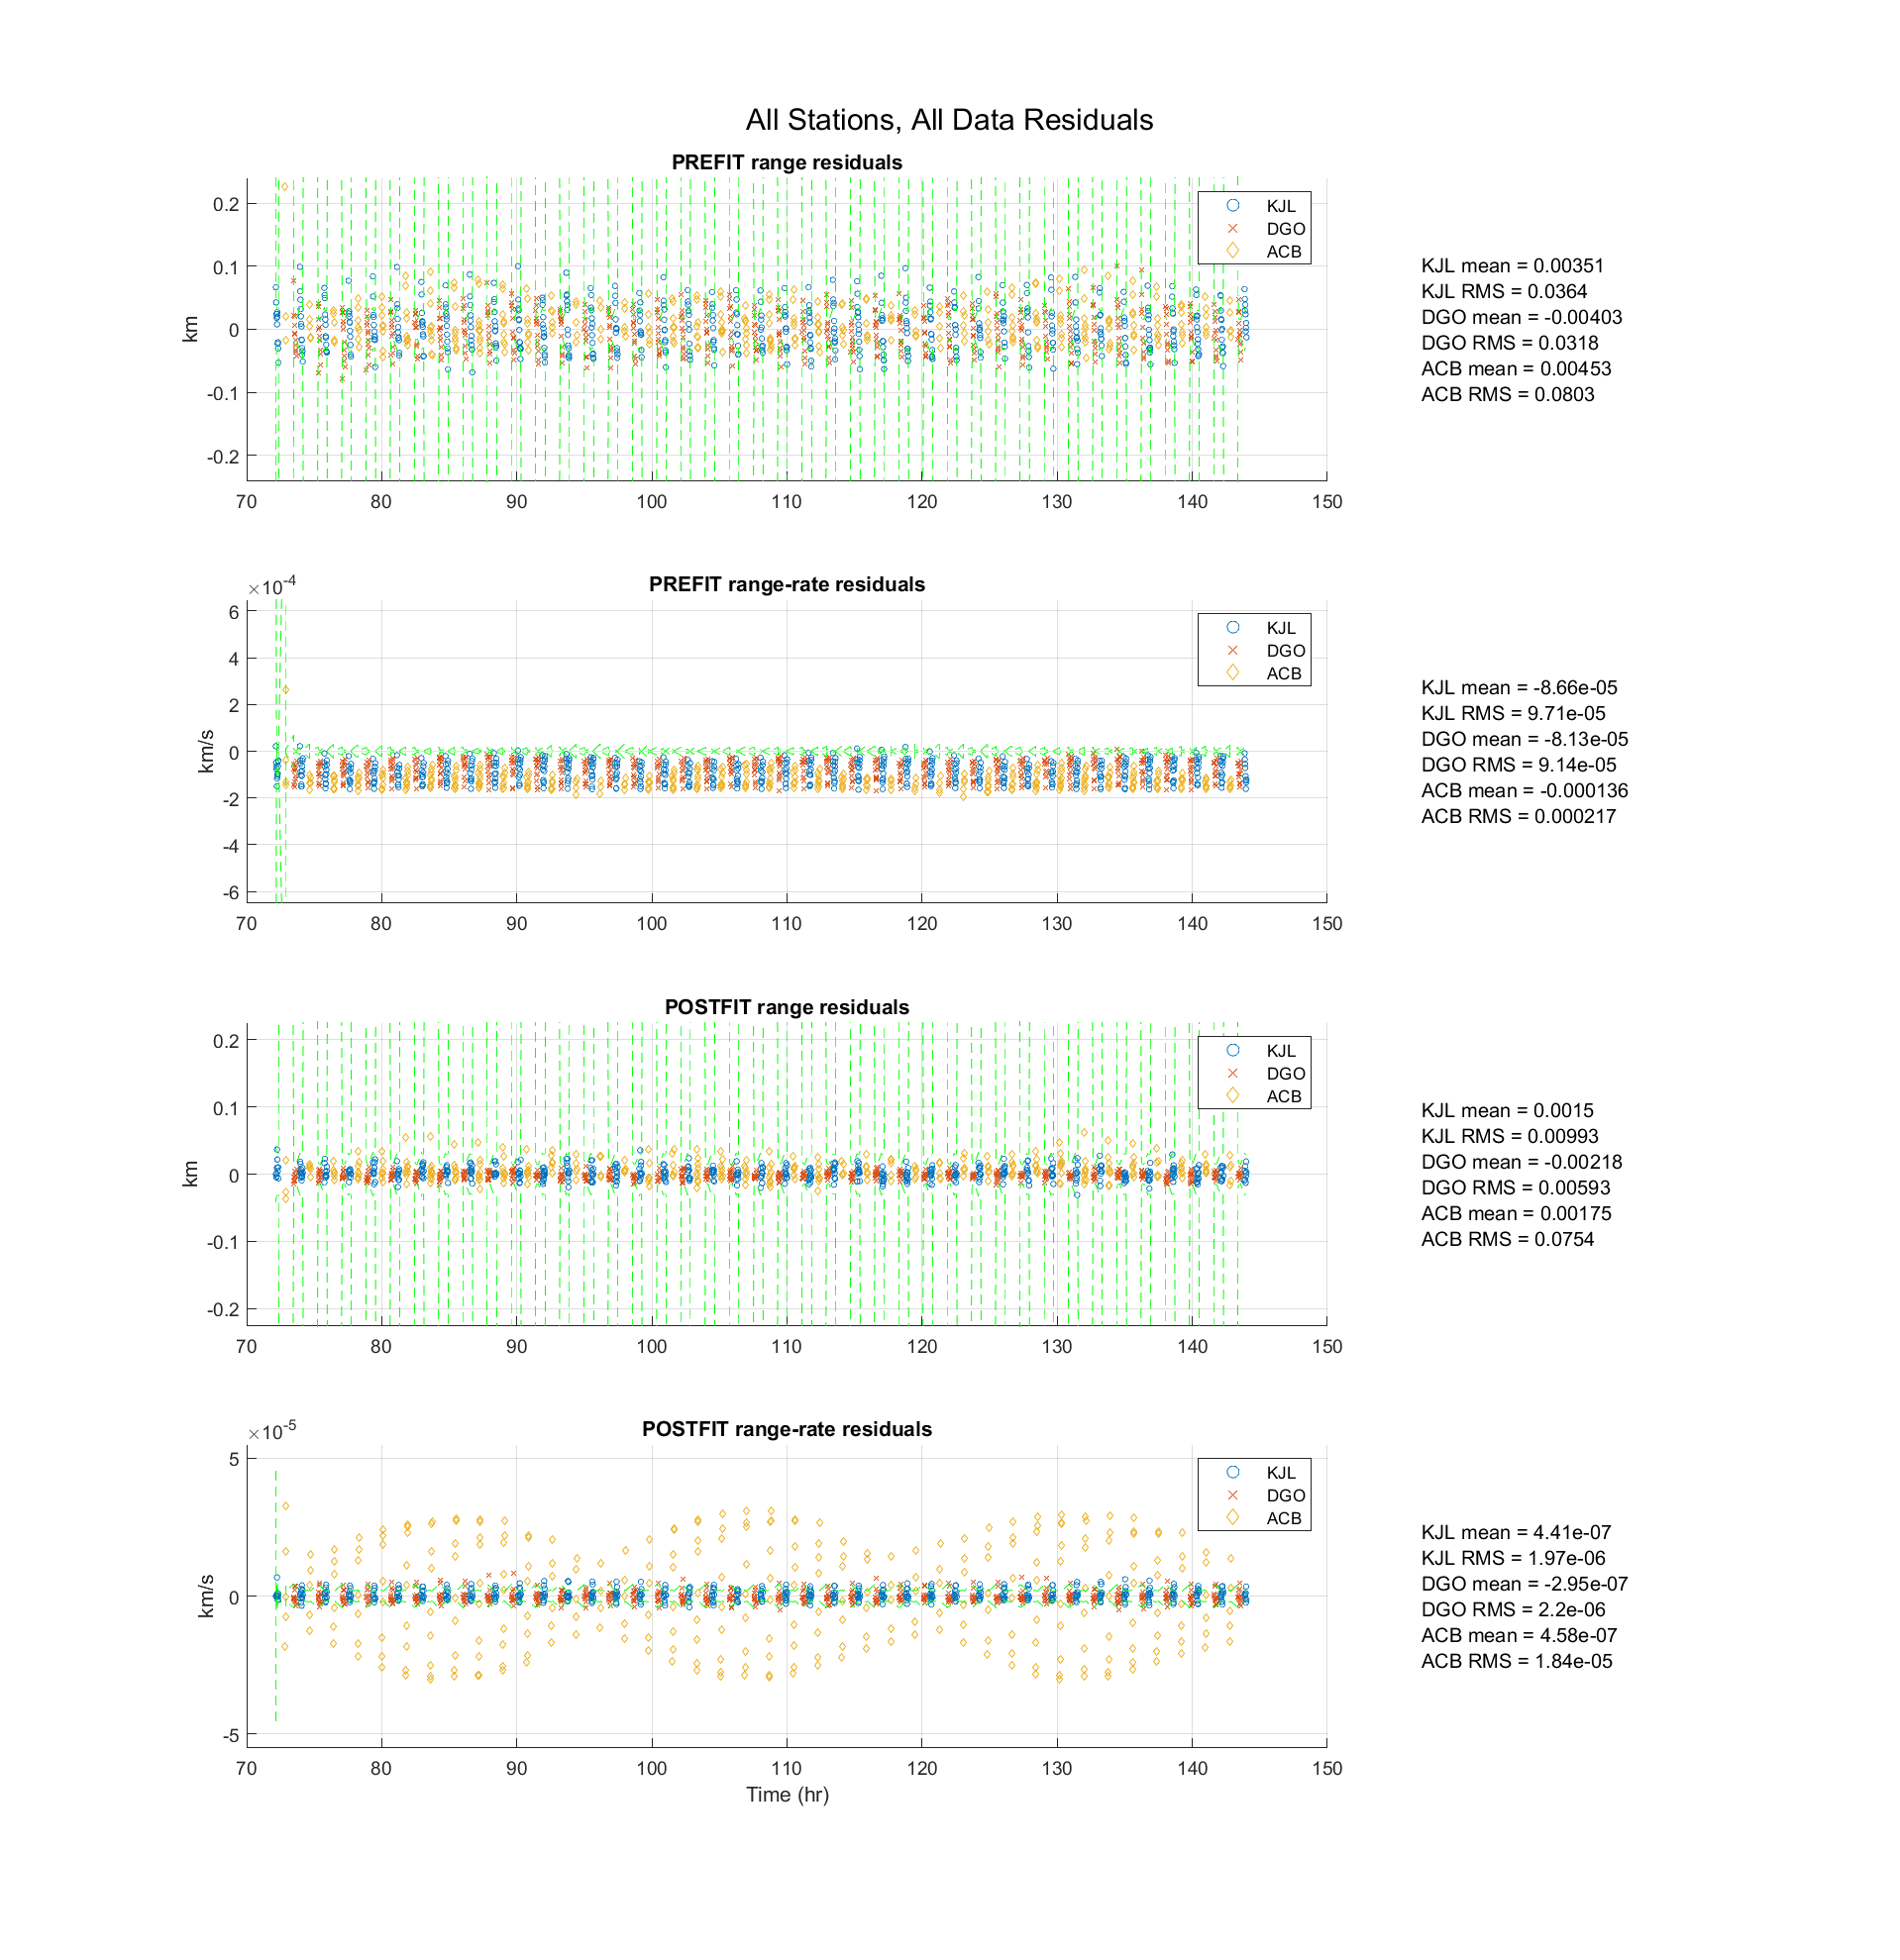
\includegraphics[width=\textwidth]{caseG_res.png}
\caption{Case G: Short-Arc Only Prefit and Postfit Residuals}
\end{figure}



% ================================================================ % 
\section*{Problem 3}

% \subsubsection*{Statement} 
\begin{center}
	\fbox{ 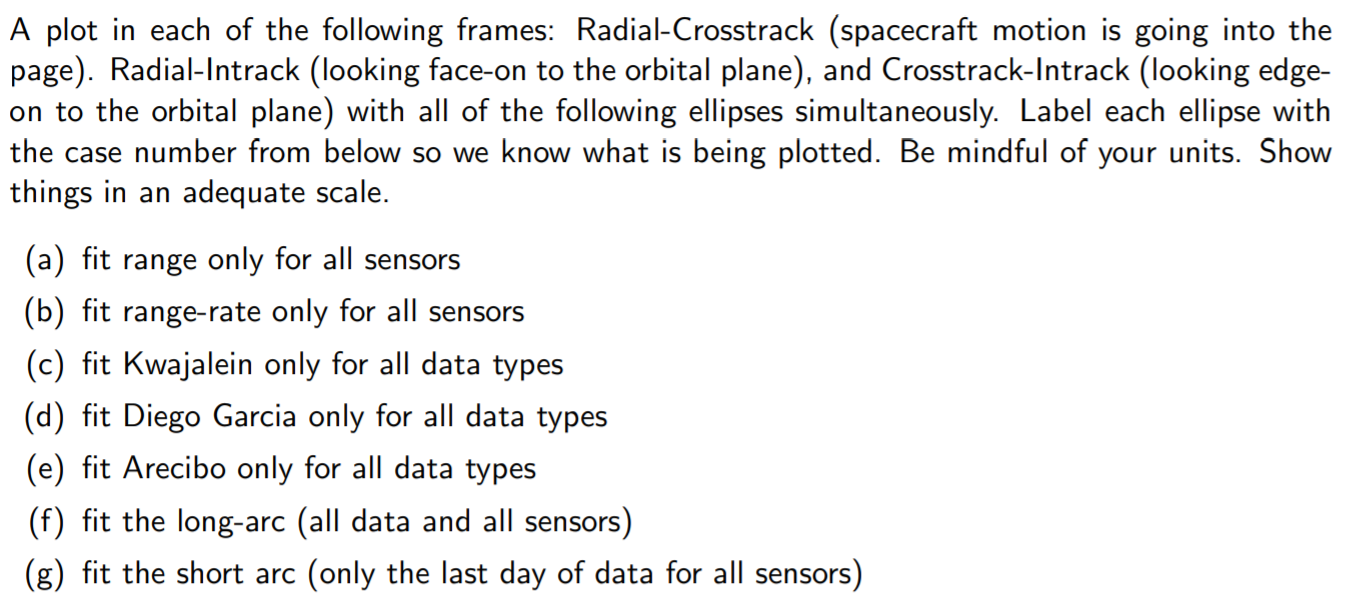
\includegraphics[width=0.8\textwidth]{prob_3.png}}
\end{center}



% ---------------------------------------------------------------- % 
\subsubsection*{Solution} 

The radial-intrack, radial-crosstrack, and intrack-crosstrack plots for Cases A - F are provided below. For Case F, the "long arc" is really just 24 hours for the first phase of this project. \textbf{The units for all axes are in kilometers.}


\begin{figure}[H]
	\centering
	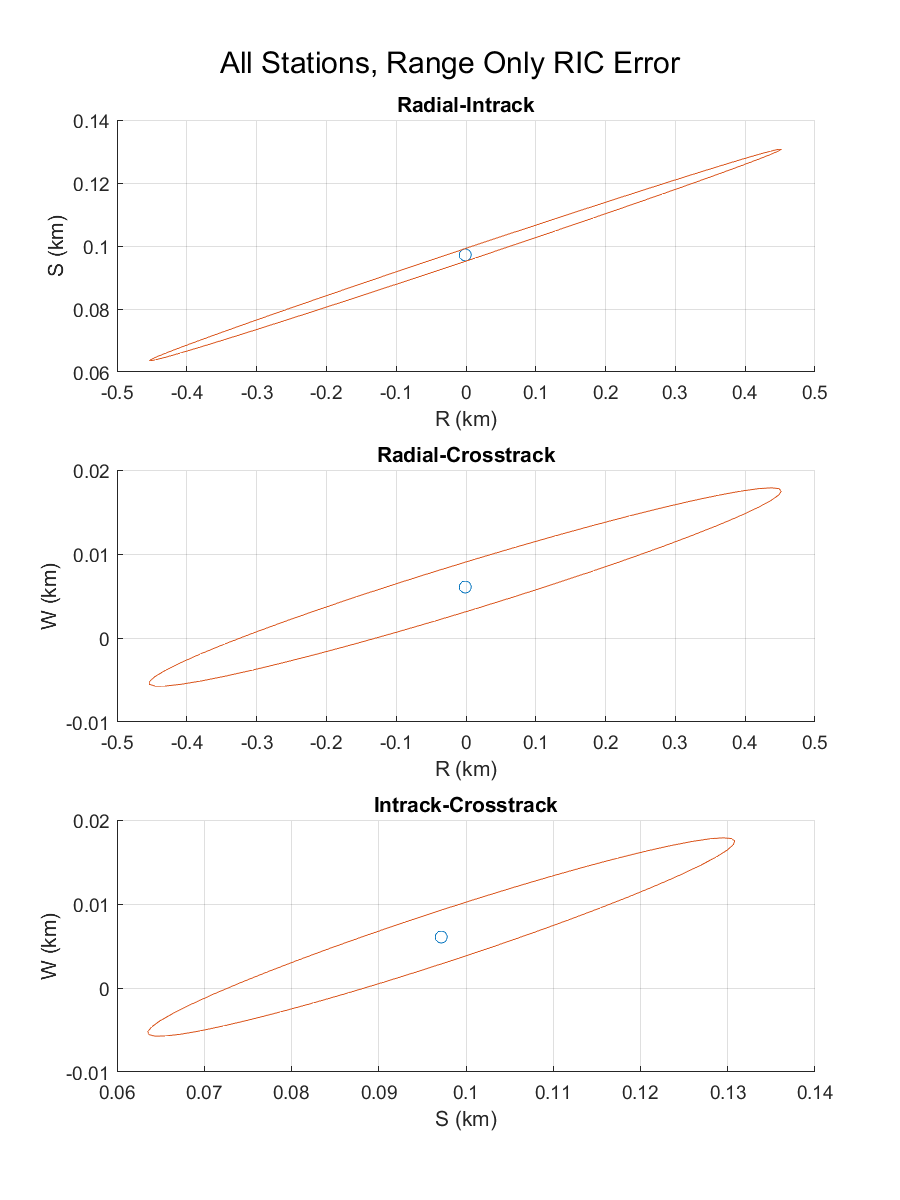
\includegraphics[width=0.7\textwidth]{caseA_RICerr.png}
	\caption{Case A: Range Only RIC Error}
\end{figure}

\begin{figure}[H]
	\centering
	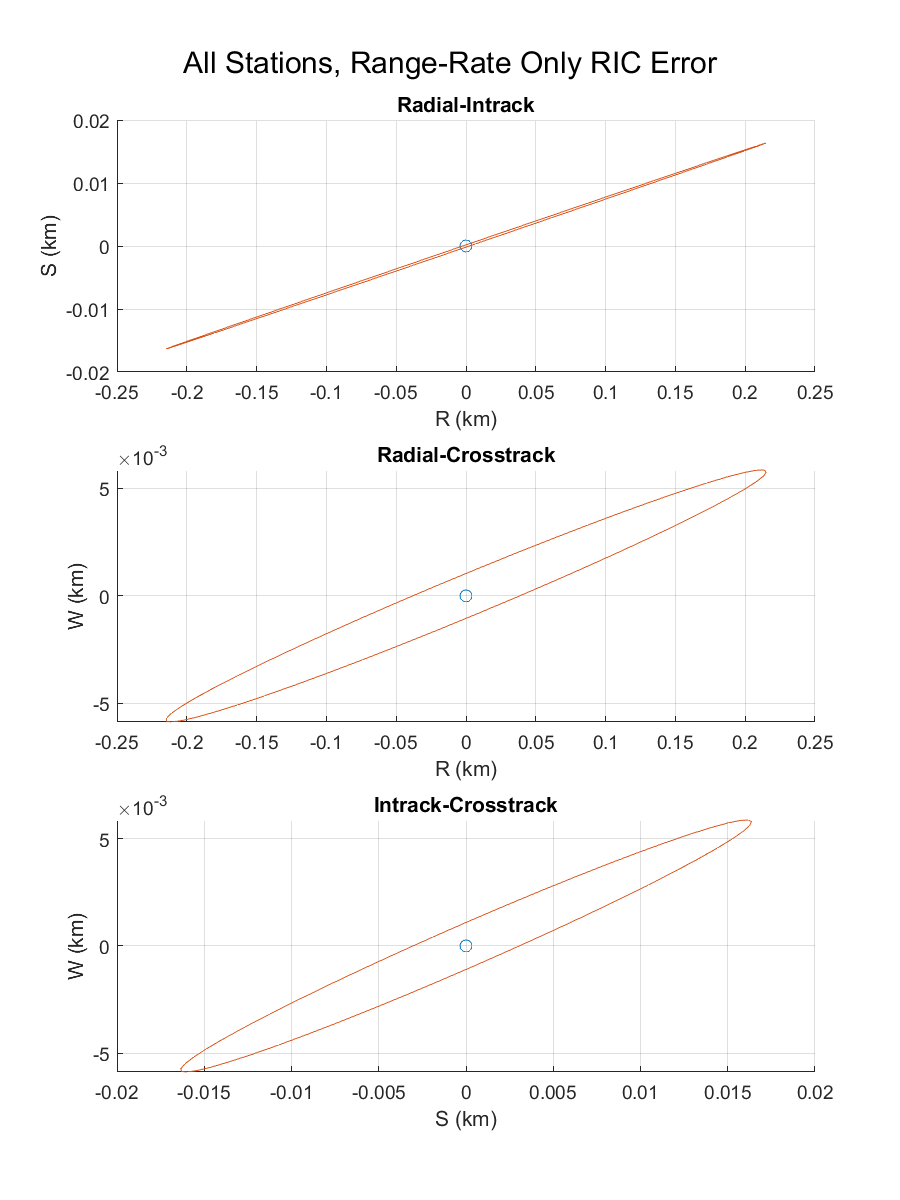
\includegraphics[width=0.7\textwidth]{caseB_RICerr.png}
	\caption{Case B: Range-Rate Only RIC Error}
\end{figure}

\begin{figure}[H]
	\centering
	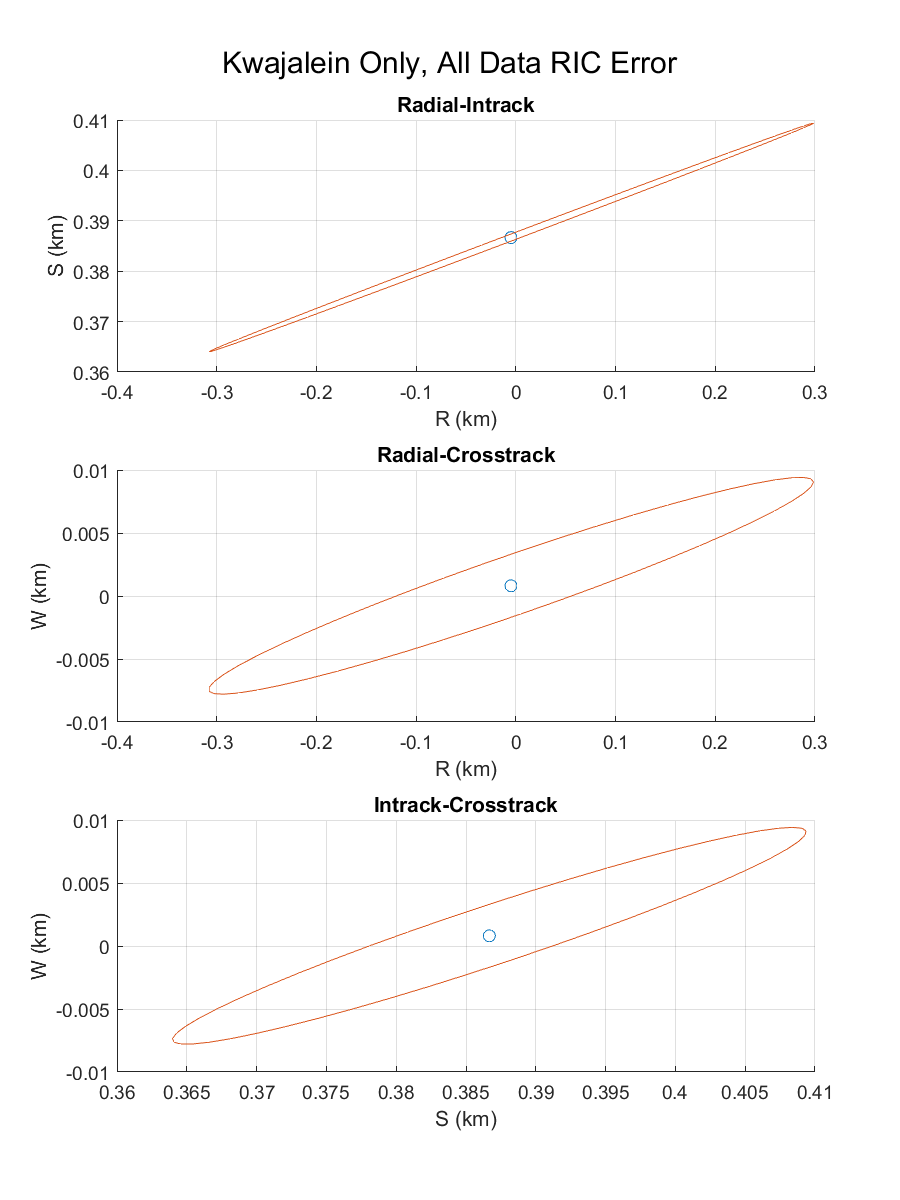
\includegraphics[width=0.7\textwidth]{caseC_RICerr.png}
	\caption{Case C: Kwajalein Only RIC Error}
\end{figure}

\begin{figure}[H]
	\centering
	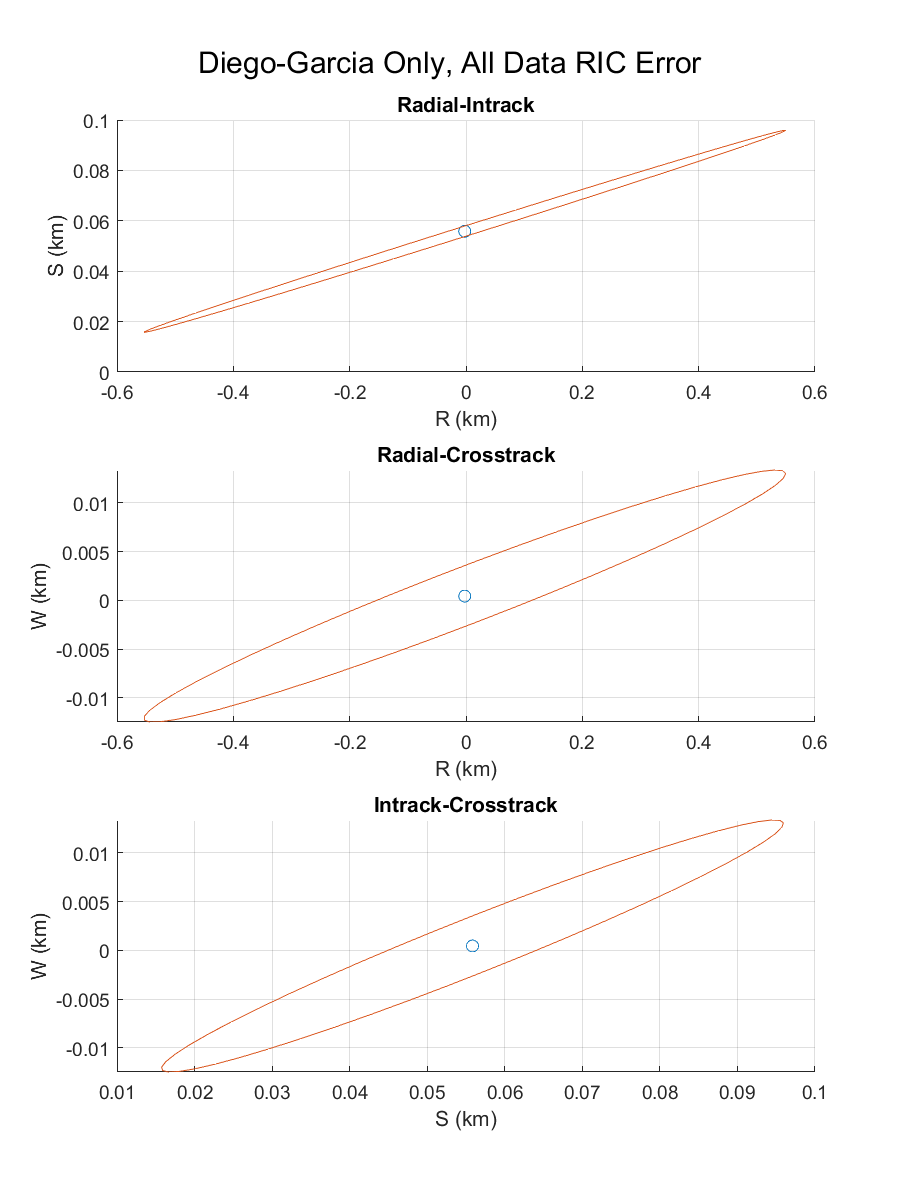
\includegraphics[width=0.7\textwidth]{caseD_RICerr.png}
	\caption{Case D: Diego Garcia Only RIC Error}
\end{figure}

\begin{figure}[H]
	\centering
	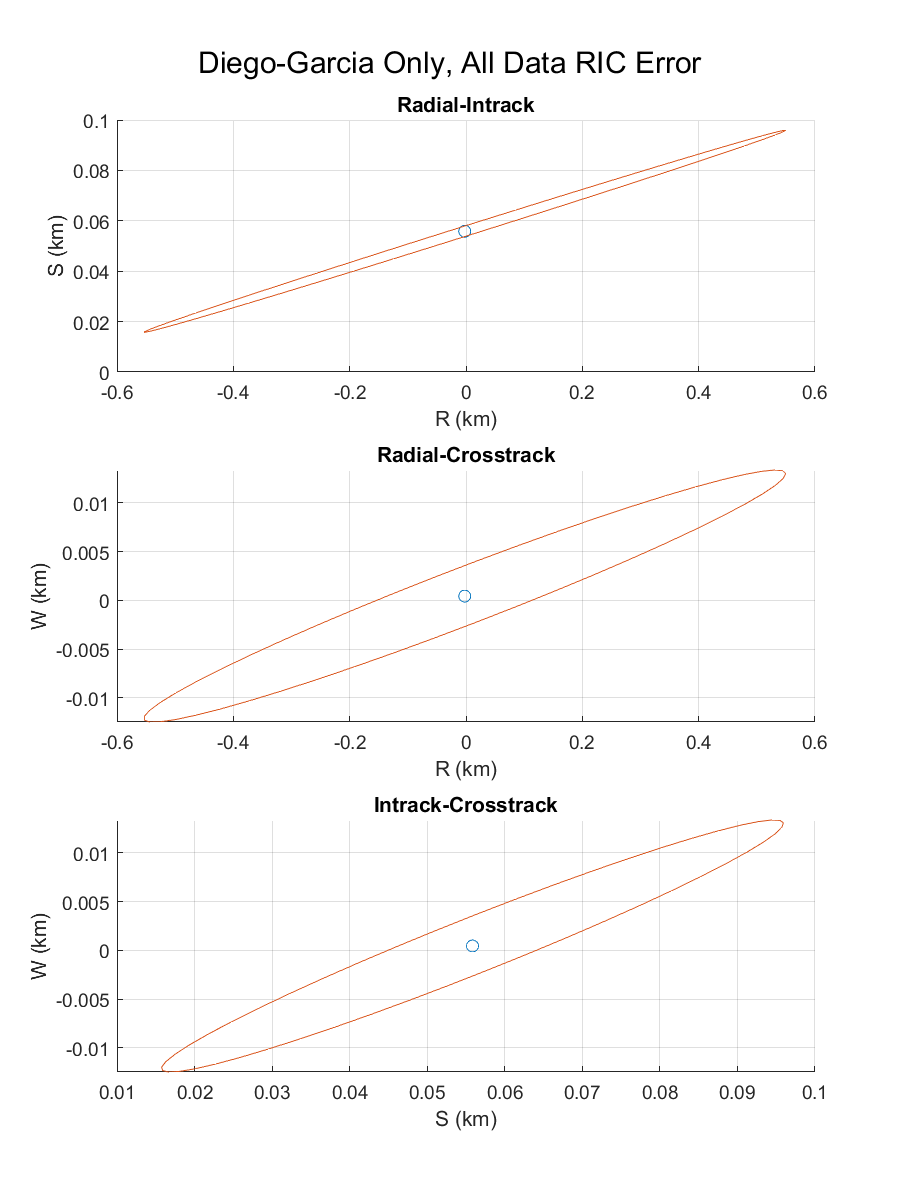
\includegraphics[width=0.7\textwidth]{caseD_RICerr.png}
	\caption{Case E: Arecibo Only RIC Error}
\end{figure}

\begin{figure}[H]
	\centering
	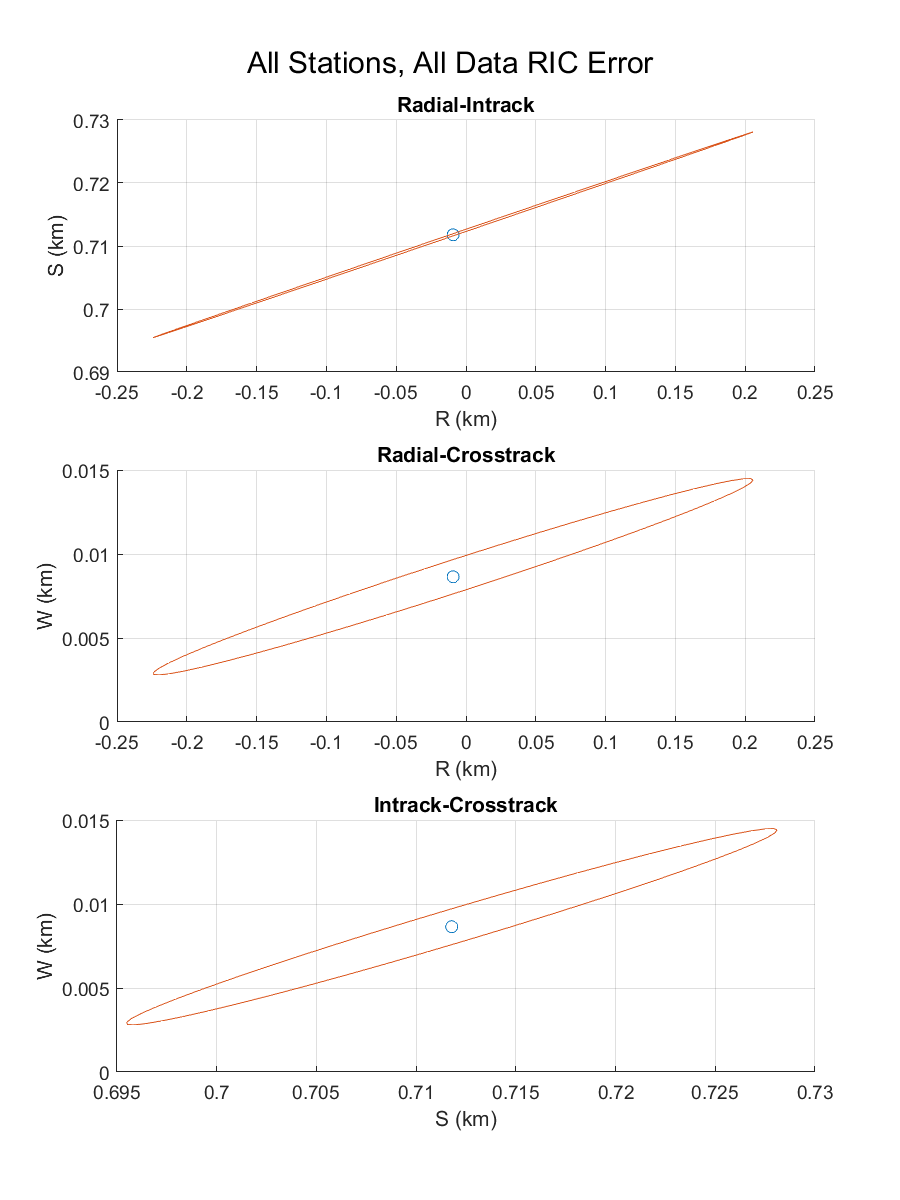
\includegraphics[width=0.7\textwidth]{caseF_RICerr.png}
	\caption{Case F: Long-Arc Only RIC Error}
\end{figure}

\begin{figure}[H]
	\centering
	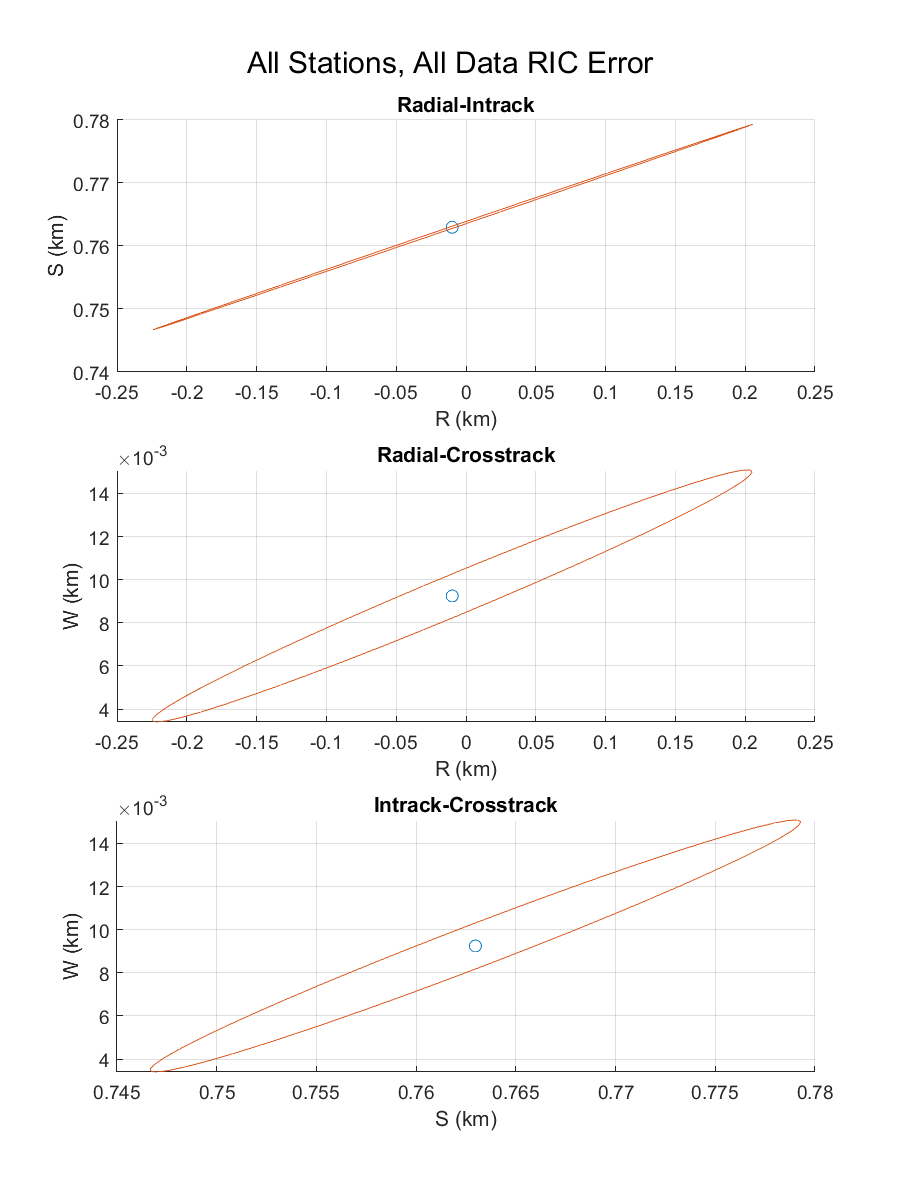
\includegraphics[width=0.7\textwidth]{caseG_RICerr.png}
	\caption{Case G: Short-Arc Only RIC Error}
\end{figure}


% ================================================================ % 
\section*{Analysis}

The final propagated states to the time of $\Delta V_1$ for each case are given below: 

% Please add the following required packages to your document preamble:
\begin{table}[H]
	\centering
	\begin{tabular}{@{}llll@{}}
		\toprule
		Case & x (km)   & y (km)    & z (km)    \\ \midrule
		Case A & 445.6184 & -7.1002e3 & -183.8598 \\
		\textbf{Case B} & \textbf{445.7151} & \textbf{-7.1002e3} & \textbf{-183.8514} \\
		Case C & 445.3296 & -7.1002e3 & -183.8615 \\
		Case D & 445.6596 & -7.1002e3 & -183.8532 \\
		Case E & 444.9273 & -7.1002e3 & -183.8699 \\
		Case F & 445.0057 & -7.1002e3 & -183.8771 \\
		Case G & 444.9547 & -7.1002e3 & -183.8789 \\ \bottomrule
	\end{tabular}
\caption{Delivery Position Estimates in ECI frame}
\end{table}

\textbf{The best estimate which should be used for the $\Delta V_1$ maneuver is Case B.}

\begin{table}[H]
	\centering
	\begin{tabular}{ c c }
		\toprule
		Case  & Position Covariance (km) \\
		\midrule \\
		\addlinespace[-2ex]
		Case A & $\begin{bmatrix}
	      	0.20514   &   0.01521    & 0.005179 \\
			0.01521   & 0.0011318  & 0.00038245 \\
			0.005179  & 0.00038245 &  0.00013953	
			 \end{bmatrix}$\\
		\addlinespace[1.5ex]
		Case B & $\begin{bmatrix}
			     0.046275   & 0.0035185  &  0.0012418 \\
			0.0035185  & 0.00026756  & 9.4283e-05 \\
			0.0012419  & 9.4283e-05  &  3.442e-05
		\end{bmatrix}$\\
		\addlinespace[1.5ex]
		Case C & $\begin{bmatrix}
			0.092019   & 0.0068838  &  0.0024976  \\
			0.0068838  & 0.00051547 &  0.00018697 \\
			0.0024976  & 0.00018697 &  7.4071e-05
		\end{bmatrix}$\\
		\addlinespace[1.5ex]
		Case D & $\begin{bmatrix}
			0.30446    & 0.022101   & 0.0069232  \\
			0.022101   & 0.0016086  & 0.00050364 \\
			0.0069234  & 0.00050366 &  0.00016723
		\end{bmatrix}$\\
		\addlinespace[1.5ex]
		Case E & $\begin{bmatrix}
      		1.1775    & 0.079641    & 0.027798   \\
			0.079639  &  0.0054069 &   0.0018739 \\
			0.0278   & 0.0018741  & 0.00067882
		\end{bmatrix}$\\
		\addlinespace[1.5ex]
		Case F & $\begin{bmatrix}
		    0.046158   & 0.0035054   & 0.0012366  \\
			0.0035054  & 0.00026624  & 9.3775e-05 \\
			0.0012366  & 9.3775e-05  & 3.4173e-05
		\end{bmatrix}$\\
		\addlinespace[1.5ex]
		Case F & $\begin{bmatrix}
	     	0.046175   & 0.0035063   &  0.001237  \\
			0.0035063  & 0.00026628  & 9.3798e-05 \\
			0.001237  & 9.3798e-05  & 3.4184e-05
		\end{bmatrix}$\\
		
		\bottomrule
	\end{tabular}
	\caption{Delivery Position Covariances in ECI frame}
\end{table}

%Provide a detailed narrative of your analyses and your interpretation of the results. What are these cases indicating to you? 

% How does each sensor and data type contribute to the overall uncertainty (knowledge and delivery)? Did you have to compensate for unmodeled dynamics? If so, how? 

% How well are you predicting future measurements? Did you infer the presence of any biases? If so, which? 

% What do you seem most sensitive to in your solutions? 

% How observable are your states and parameters? 

% What did you estimate? Did you ”consider’ any parameters? 

% Did you smooth the trajectory? If so, how did this help? 

% What was your strategy for getting your results and making it all ”work?”

%Be explicit in listing all of your assumptions as these should always caveat your analyses. Some of them follow (i.e. initial conditions, a priori uncertainty, observation model(s) used, dynamic model(s) used, spacecraft model(s) used, states and parameters estimated and/or considered, process noise model(s) used, estimation strategy used [e.g. EKF, batch, UKF, etc.]). 

% Provide a rationale for why you chose what you did and not something else, for instance. Orbit Determination and Prediction is a science and also an art with its own ”tradecraft.” Part of your evaluation is based upon this tradecraft that you developed over the course.


\subsection{Dynamic Model}

The spacecraft dynamics model incorporated perturbations due to spherical harmonics, lunisolar effects, solar radiation pressure, and atmospheric drag. 

\subsubsection{Gravity Model}

The spherical harmonics model used was GGM03S, which is derived purely on 4 years of highly accurate data from the GRACE satellite (from January 2003 to December 2006), truncated to 20 degree and order. EGM2008, the spherical harmonic model released by the National Geospatial-Intelligence Agency in 2008, combines the long wavelength GRACE data with global 5 arc-minute equiangular grid of area-mean free-air gravity anomalies. 

The gravitational coefficients for the gravity spherical harmonics model were taken from GGM03S, which is available on the GRACE website \cite{GRACE}. The gravitational potential function in the form derived by Levinson is \cite{levinson_gravity}: 

\begin{equation}
	V = \dfrac{GM}{r} \Bigg\{ 1 + \sum_{n_max}^{n=2} \bigg[ 
	\bigg( \frac{a}{r} \bigg)^n \sum_{m=0}^{n} \bar{P}_{n,m}(sin \beta) ( \bar{C}_{n,m} cos m \lambda + \bar{S}_{n,m} sin m \lambda )
	 \bigg] \Bigg\}
\end{equation}
\label{eq:gravity}

where G is the universal gravitational constant, M is the mass of the Earth, n is the order, m is the degree, $\beta$ is the longitude, $\lambda$ is the latitude, $\bar{P}$ is a normalized associated Legendre function based on the degree and order, and $\bar{C}$ and $\bar{S}$ are normalized gravitational coefficients from GGM03S. To produce the spacecraft accelerations $\Delta V$, Equation \ref{eq:gravity} was differentiated with respect to r, $\lambda$, and $\beta$ and substituted into the following equation, where $\hat{x}$, $\hat{y}$, and $\hat{z}$ are the orthogonal basis unit vectors for the ECI frame: 

\begin{equation}
	\Delta V = 
	\bigg( \dfrac{\delta V}{\delta r} cos \beta cos \lambda - \dfrac{\delta V}{\delta \lambda} \dfrac{sin \lambda}{ r cos \beta } - \dfrac{\delta V}{\delta \beta } \dfrac{sin \beta cos \lambda }{r } \bigg) \hat{x} + 
	\bigg( \dfrac{\delta V}{\delta r} cos \beta sin \lambda - \dfrac{\delta V}{\delta \lambda} \dfrac{cos \lambda}{ r cos \beta } - \dfrac{\delta V}{\delta \beta } \dfrac{sin \beta sin \lambda }{r } \bigg) \hat{y} + 
	\bigg( \dfrac{\delta V}{\delta r} sin \beta + \dfrac{\delta V}{\delta \beta} \dfrac{cos \beta}{r} \bigg) \hat{z} 	
\end{equation} 

To compute the A matrix of partial derivatives, only the zonal terms J2, J3, and J4 were considered, in which n = 2, 3, 4; and m = 0. 

\subsubsection{Lunisolar Effects}

Lunisolar effects were modeled as third-body gravitational perturbations. The perturbing force contribution according to Born is \cite{born_statorbitdet}: 

\begin{equation}
	f_{3B} = \sum_{j=1}^{n_p} \mu_j \bigg( \dfrac{\pmb{\Delta}_{j}}{\Delta_j^3} - \dfrac{\pmb{r}_j}{r_j^3} \bigg)
\end{equation}

where $n_p$ is the number of additional bodies, $j$ represents a specific body such as the sun or the moon, $\mu_j$ is the gravitational parameter of the specific body, $\pmb{\Delta}_j$ is the position vector of the body with respect to the satellite, and $\pmb{r}_j$ is the position vector of the body with respect to the Earth. 

SPICE was used to find the position vectors of the third bodies in the J2000 frame using \texttt{naif0011.tls}, \texttt{de421.bsp}, and \texttt{pck00010.tpc}, all of which are available to download on the SPICE website \url{https://naif.jpl.nasa.gov/naif/toolkit.html}. 

\subsubsection{Solar Radiation Pressure}

The method for computing solar radiation pressure (SRP) was taken from \cite{vallado}. The SIGHT algorithm was used to check whether the Sun is lighting the satellite (pg. 308), which uses line-of-sight (LOS) geometry to check if the sum of the angles of the Earth to satellite and the Earth to Sun is larger than a requisite minimum angle for LOS. 

If LOS exists, then the equation to find solar radiation pressure is calculated as:

\begin{equation}
	a_{srp} = - \sum_{i = 1} \dfrac{p_{srp} A_i cos (\theta_{inc_i}) }{m} \bigg\{ 2 \bigg( \dfrac{c_{Rd_i}}{3} + c_{Rs}_i cos(\theta_{inc_i}) \bigg) \hat{n} + ( 1 - c_{Rs_i} ) \hat{s} \bigg\} 
\end{equation} 

where $p_{srp}$ is the incoming solar pressure, $\theta_{inc}$ is the angle between the surface normal and incoming radiation (in direction of sun vector), m is the satellite mass, $c_{Rd}$ is the diffuse reflectivity, $c_{Rs}$ is the specular reflectivity, $\hat{n}$ is the surface normal vector, and $\hat{s}$ is the sun vector from the Earth to the sun direction. 

The SRP due to different coatings on each face was modeled. The surface normals of the local spacecraft x, y, and z axes were calculated in the ECI frame, and the specific specular and diffuse reflectivity applied for whether it was the positive or negative face illuminated. 

If LOS does not exist, then the SRP is zero. 

\subsubsection{Atmospheric Drag}

The drag model is relatively simple compared to the other modeled perturbation effects and was taken from Born \cite{born_statorbitdet}: 

\begin{equation}
	a_{drag} = -1/2 \rho \big( \dfrac{C_D A}{m} \big) V_r \pmb{V}_r
\end{equation}

where $\rho$ is the atmospheric density, $C_D$ is the drag coefficient, $\pmb{V}_r$ is the vehicle velocity relative to the atmosphere, A is the cross-sectional area, and m is the mass. Only the drag on the solar panel was accounted for in the drag model. 

\subsection{Estimation Process}

The measurement data was smoothed using a batch processor and Extended Kalman Filter. The batch processor was used to improve the approximated initial state of the satellite and the Extended Kalman Filter (EKF) was used to sequentially process the measurement data up to the final day of dynamic propagation for $\Delta V_1$. The EKF was chosen due to its flexibility with nonlinear systems and computational efficiency. The EKF is also aided by having a better initial state which is provided by the batch processor. 

Both filtering methods were taken from Born \cite{born_statorbitdet}. All position and range units are in kilometers and all velocity and range-rate units are in kilometers/second. 

To set up both filters, the following measurement covariances were used for each station: 

\begin{equation}
	R_{KJL} = 
	\begin{bmatrix}
		(10e-3)^2 & 0 \\ 
		0 & (0.5e-6)^2
	\end{bmatrix}
\end{equation}

\begin{equation}
	R_{DGO} = 
	\begin{bmatrix}
		(5e-3)^2 & 0 \\ 
		0 & (1e-6)^2
	\end{bmatrix}
\end{equation}

\begin{equation}
	R_{ACB} = 
	\begin{bmatrix}
		(10e-3)^2 & 0 \\ 
		0 & (0.5e-6)^2
	\end{bmatrix}
\end{equation}

in which KJL is Kwajalein, DGO is Diego Garcia, and ACB is Arecibo. The state covariance was initialized for position error for 10 km and velocity error of 10 m/s: 

\begin{equation}
	P_0 = 
	\begin{bmatrix}
		10^2I_{3x3} & 0_{3x3} \\
		0_{3x3} & (10^{-3})^2I_{3x3} 
	\end{bmatrix}
\end{equation}

The state for filters was the same as the state for the dynamic equations of motion, which is a [6x1] vector containing the satellite position ([3x1] km) and velocity ([3x1] km/s) in ECI frame. 

\subsubsection{Batch Processor}

The batch processor filtered through the first 28 measurements to arrive at the following initial state. As stated above, the algorithm was taken from Born (pg. 196): 

\begin{equation}
	X_0 = 
	\begin{bmatrix}
		6978.25613502827 \\
		1616.30084111326 \\
		19.7187226552466 \\
		-1.66208631750821 \\
		7.26104887569659 \\
		0.270612922289392 
	\end{bmatrix}
\end{equation}

\subsubsection{Extended Kalman Filter}

The EKF was used to produce the delivery estimates for each case. For cases using data from only one station, the covariances for unused stations were blown up by 1e10. As stated in the previous section, the algorithm was taken from Born\cite{born_statorbitdet} (pg. 212). 

Process noise was used to compensate for unmodeled dynamics. The process noise Q used in the EKF for each measurement update was: 

\begin{equation}
	Q = \begin{bmatrix}
		(10e-10)^2	& 0 & 0 \\ 
		0 & (10e-10)^2 & 0 \\ 
		0 & 0 & (10e-10)^2
	\end{bmatrix}
\end{equation} 

Experimenting with increasing and lowering the process noise and how it affected the delivery accuracy led to the above values. Some amount of process noise was applied to the RIC frame for the \textbf{final propagation process } with the below process noise, but it did not affect the final position delivery estimate, only increasing the uncertainty covariance. I was wary of adding too much artificial process noise and used a delta-time of 60 seconds for applying RIC process noise: 

\begin{equation}
	Q_{RIC} = \begin{bmatrix}
		(100e-10)^2	& 0 & 0 \\ 
		0 & (10e-10)^2 & 0 \\ 
		0 & 0 & (100e-10)^2
	\end{bmatrix}
\end{equation}

Lighttime and bias correction were used in the EKF. The following figure  illustrates how lighttime and stellar aberration affect station measurements: 

\begin{figure}[H]
	\centering
	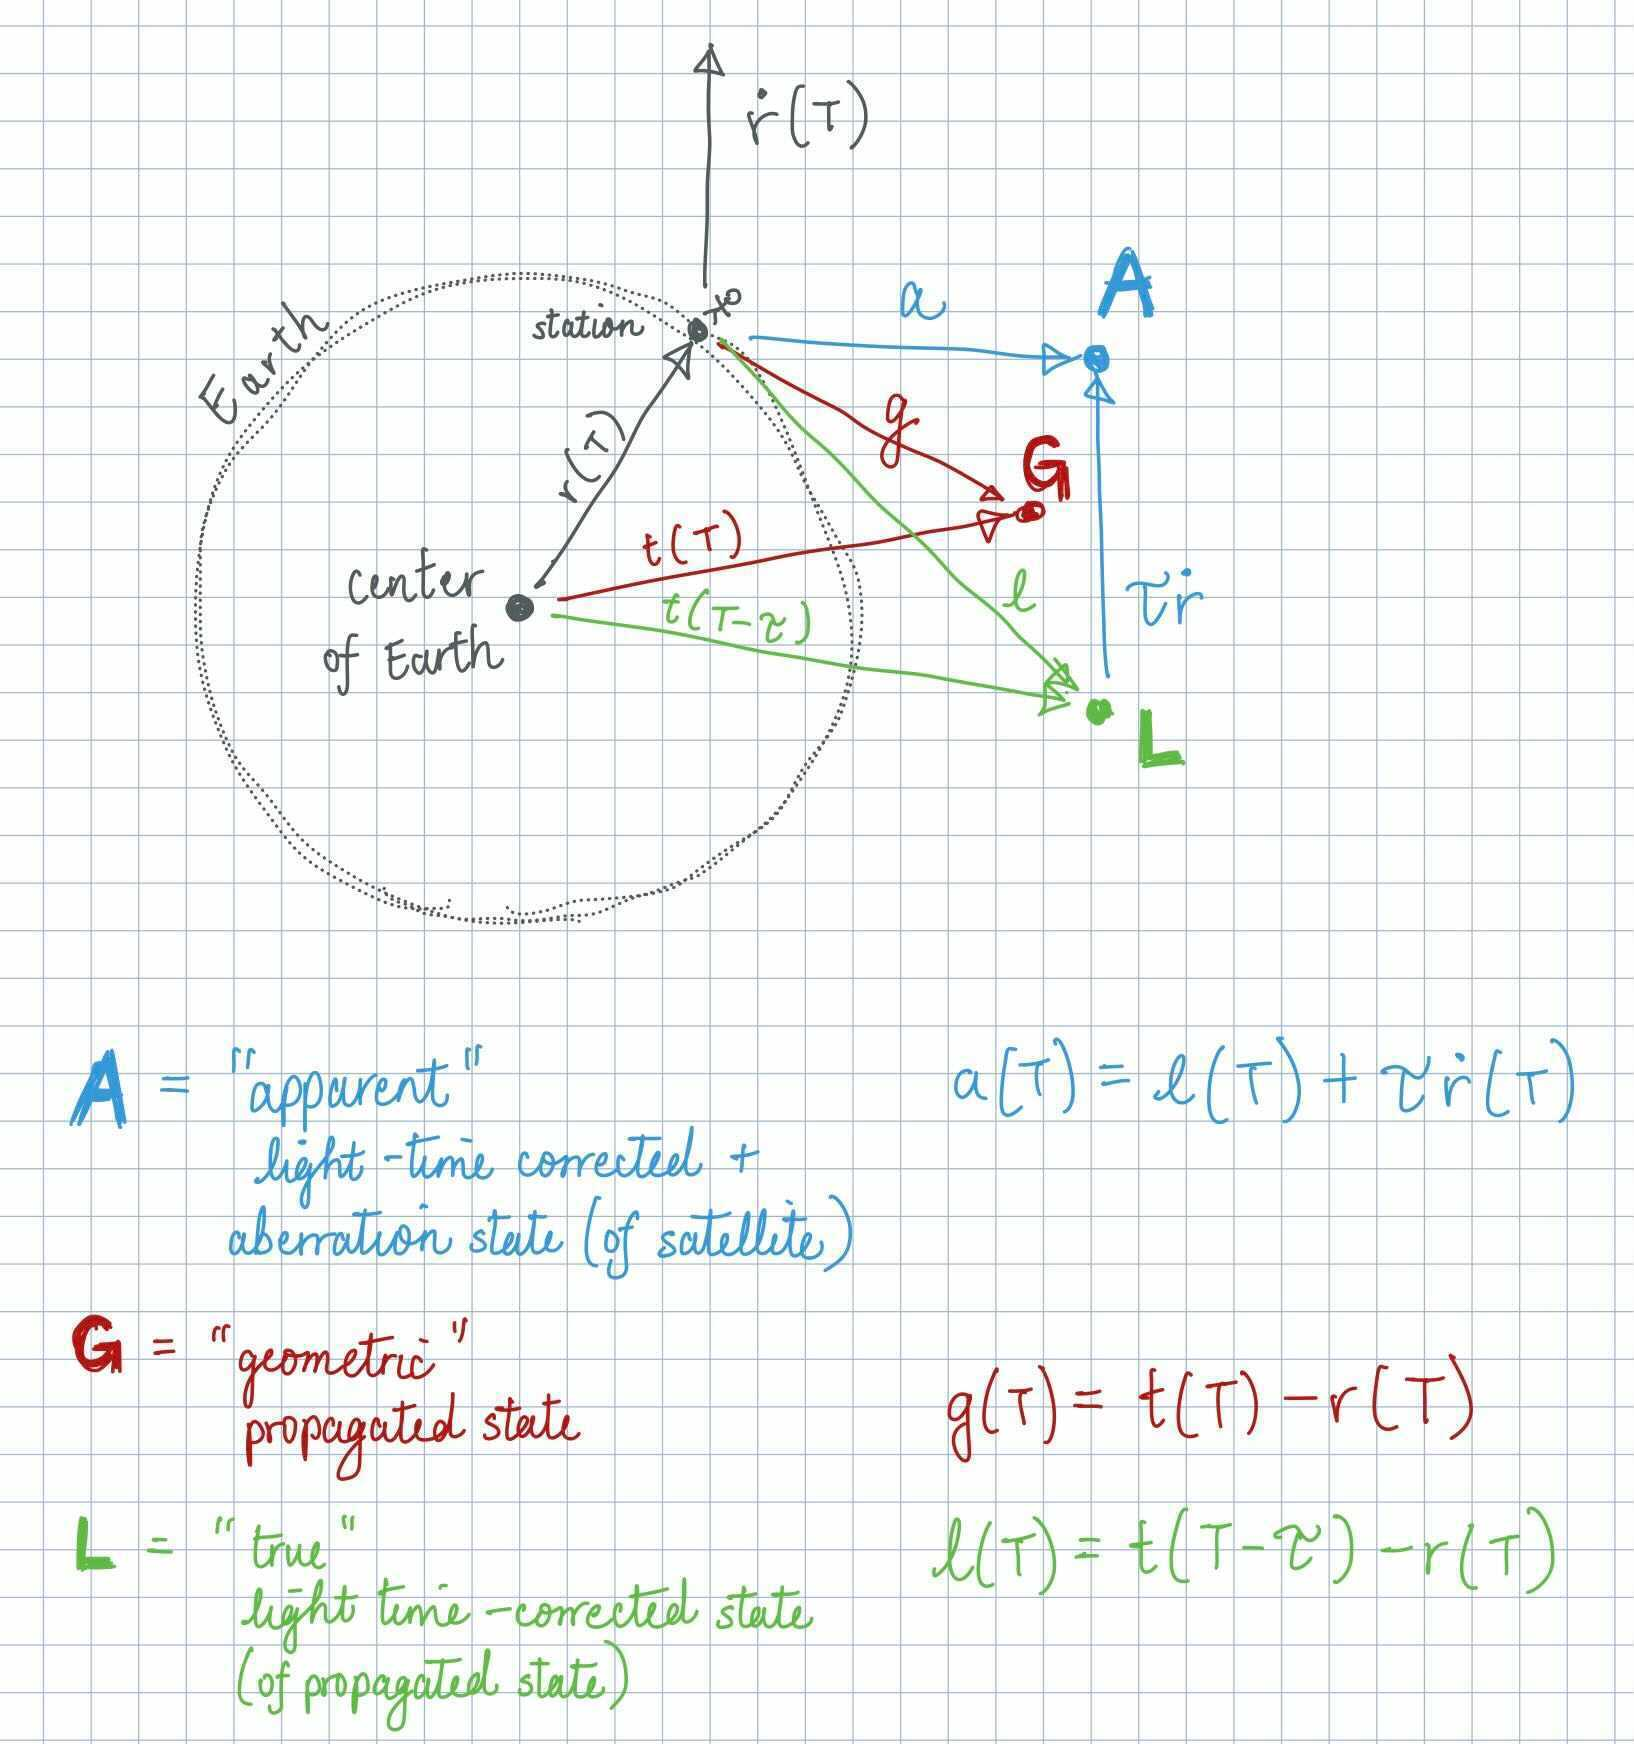
\includegraphics[width=0.5\textwidth]{lt_aberr.jpg}
	\label{fig:lt_aberr}
\end{figure}

The light time correction was found by dividing the range measurement by the speed of light and subtracting the time of the propagated satellite state with the light time correction. The state was then back-propagated to the corrected time. 

Aberration effect can be calculated by multiplying the light-time correction (a delta time) with the velocity of the station in ECI frame, and then adding the result to the back-propagated state. I tried incorporating aberration effects but it resulted in a delivery result that was more incorrect. It is possible that this is due to my ECEF to ECI function, whose implementation was taken from Vallado (the reference frames transformations methodology I used was explored in  Homework 4 \cite{HW4}). I was unable to debug this phenomenon in time and thus left aberration effects out of the EKF. 

Bias was found by running the all stations, all data case and observing the postfit residual means. figure \ref{fig:nobias} shows a day's worth of filtering with no modeled bias effects (although at the time of creating this figure, no modeled light time or aberration effects either). The Kwajalein and Diego Garcia range residuals are almost zero-mean, but the Arecibo range residual mean is 1 to 2 orders of magnitude larger than the other stations. The Arecibo mean found through this analysis was 0.0209 km. Dr. Jah later revealed in the course that the Arecibo mean is actually 0.020 km. The prefit and postfit residuals plotted in the first section use the correct bias for Arecibo. 

\begin{figure}[H]
	\centering
	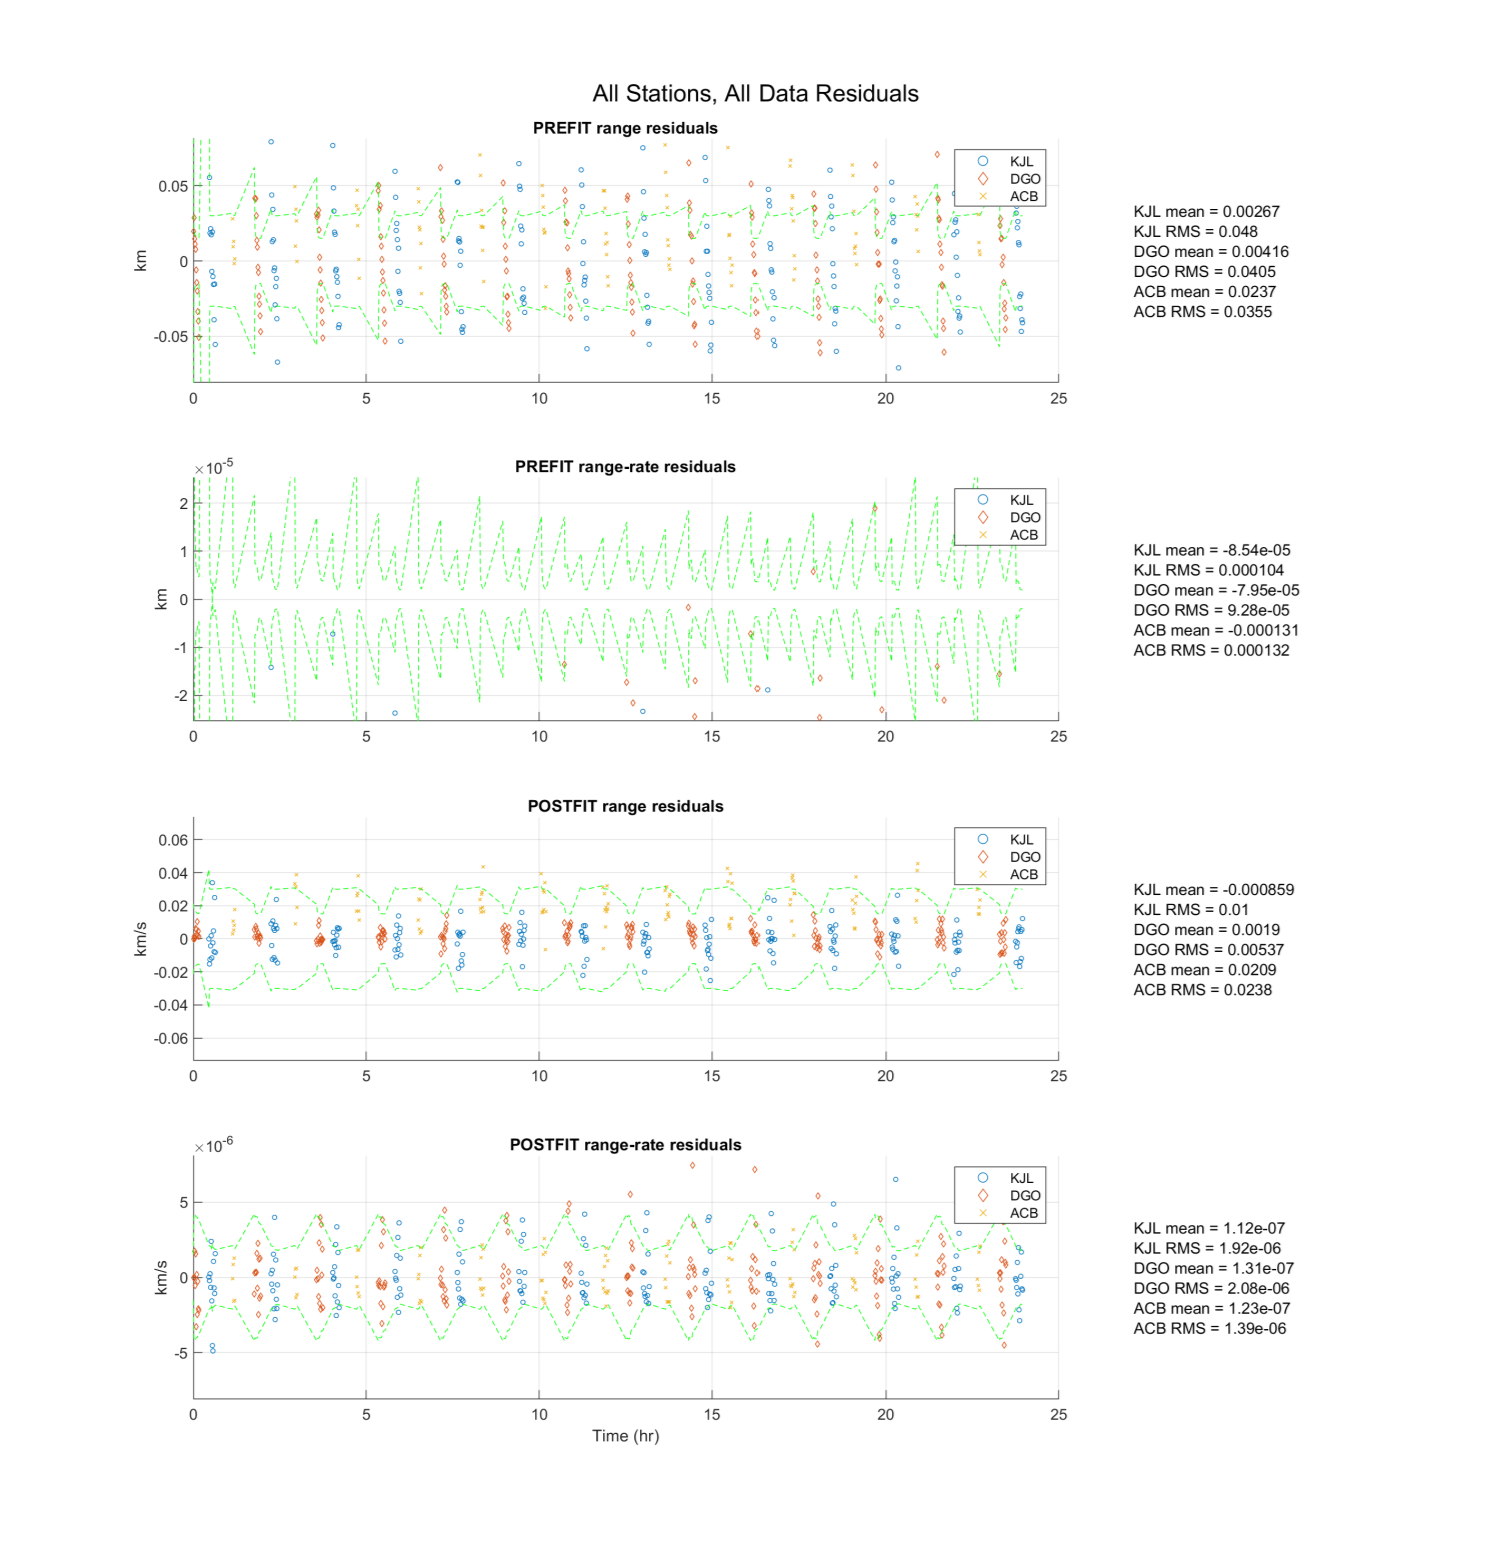
\includegraphics[width=0.8\textwidth]{allsta_alldata_nobias.png}
\end{figure}
\label{fig:nobias}

The measurement model was updated with bias for Arecibo, which included updating the G function and the H function, which is the partial derivative of the G function with respect to the satellite state. \textbf{The correct way to implement bias would be to add the station bias to the measurement model range calculation, however this led to more inaccurate results.} Instead, I was able to achieve better results by subtracting, not adding the bias, as shown below on line 17. 

\begin{lstlisting}
	function y = G_bias_fn(X, XS, STA)
	% X  = satellite coords (SAME COORD)
	% XS = station coords (SAME COORD)
	
	KJL_rbias = 0;  
	DGO_rbias = 0; 
	% ACB_rbias = 0; 
	ACB_rbias = 0.020; 
	
	if      STA == 1;   rbias = KJL_rbias;   
	elseif  STA == 2;   rbias = DGO_rbias;   
	elseif  STA == 3;   rbias = ACB_rbias;   
	end
	
	r_site = [X(1)-XS(1); X(2)-XS(2); X(3)-XS(3)]; 
	v_site = [X(4)-XS(4); X(5)-XS(5); X(6)-XS(6)]; 
	d      = norm(r_site) - rbias; 
	v      = dot(v_site, r_site / d); 
	
	y      = [d; v]; 
	
	end 
\end{lstlisting}

Another consequence of updating the measurement model to include bias was that the RMS of the range-rate residuals for Arecibo became larger by an order of magnitude, as shown below. Compare the POSTFIT range-rate residuals in Figure \ref{fig:yesbias} (below) with Figure \ref{fig:nobias}: 

\begin{figure}[H]
	\centering
	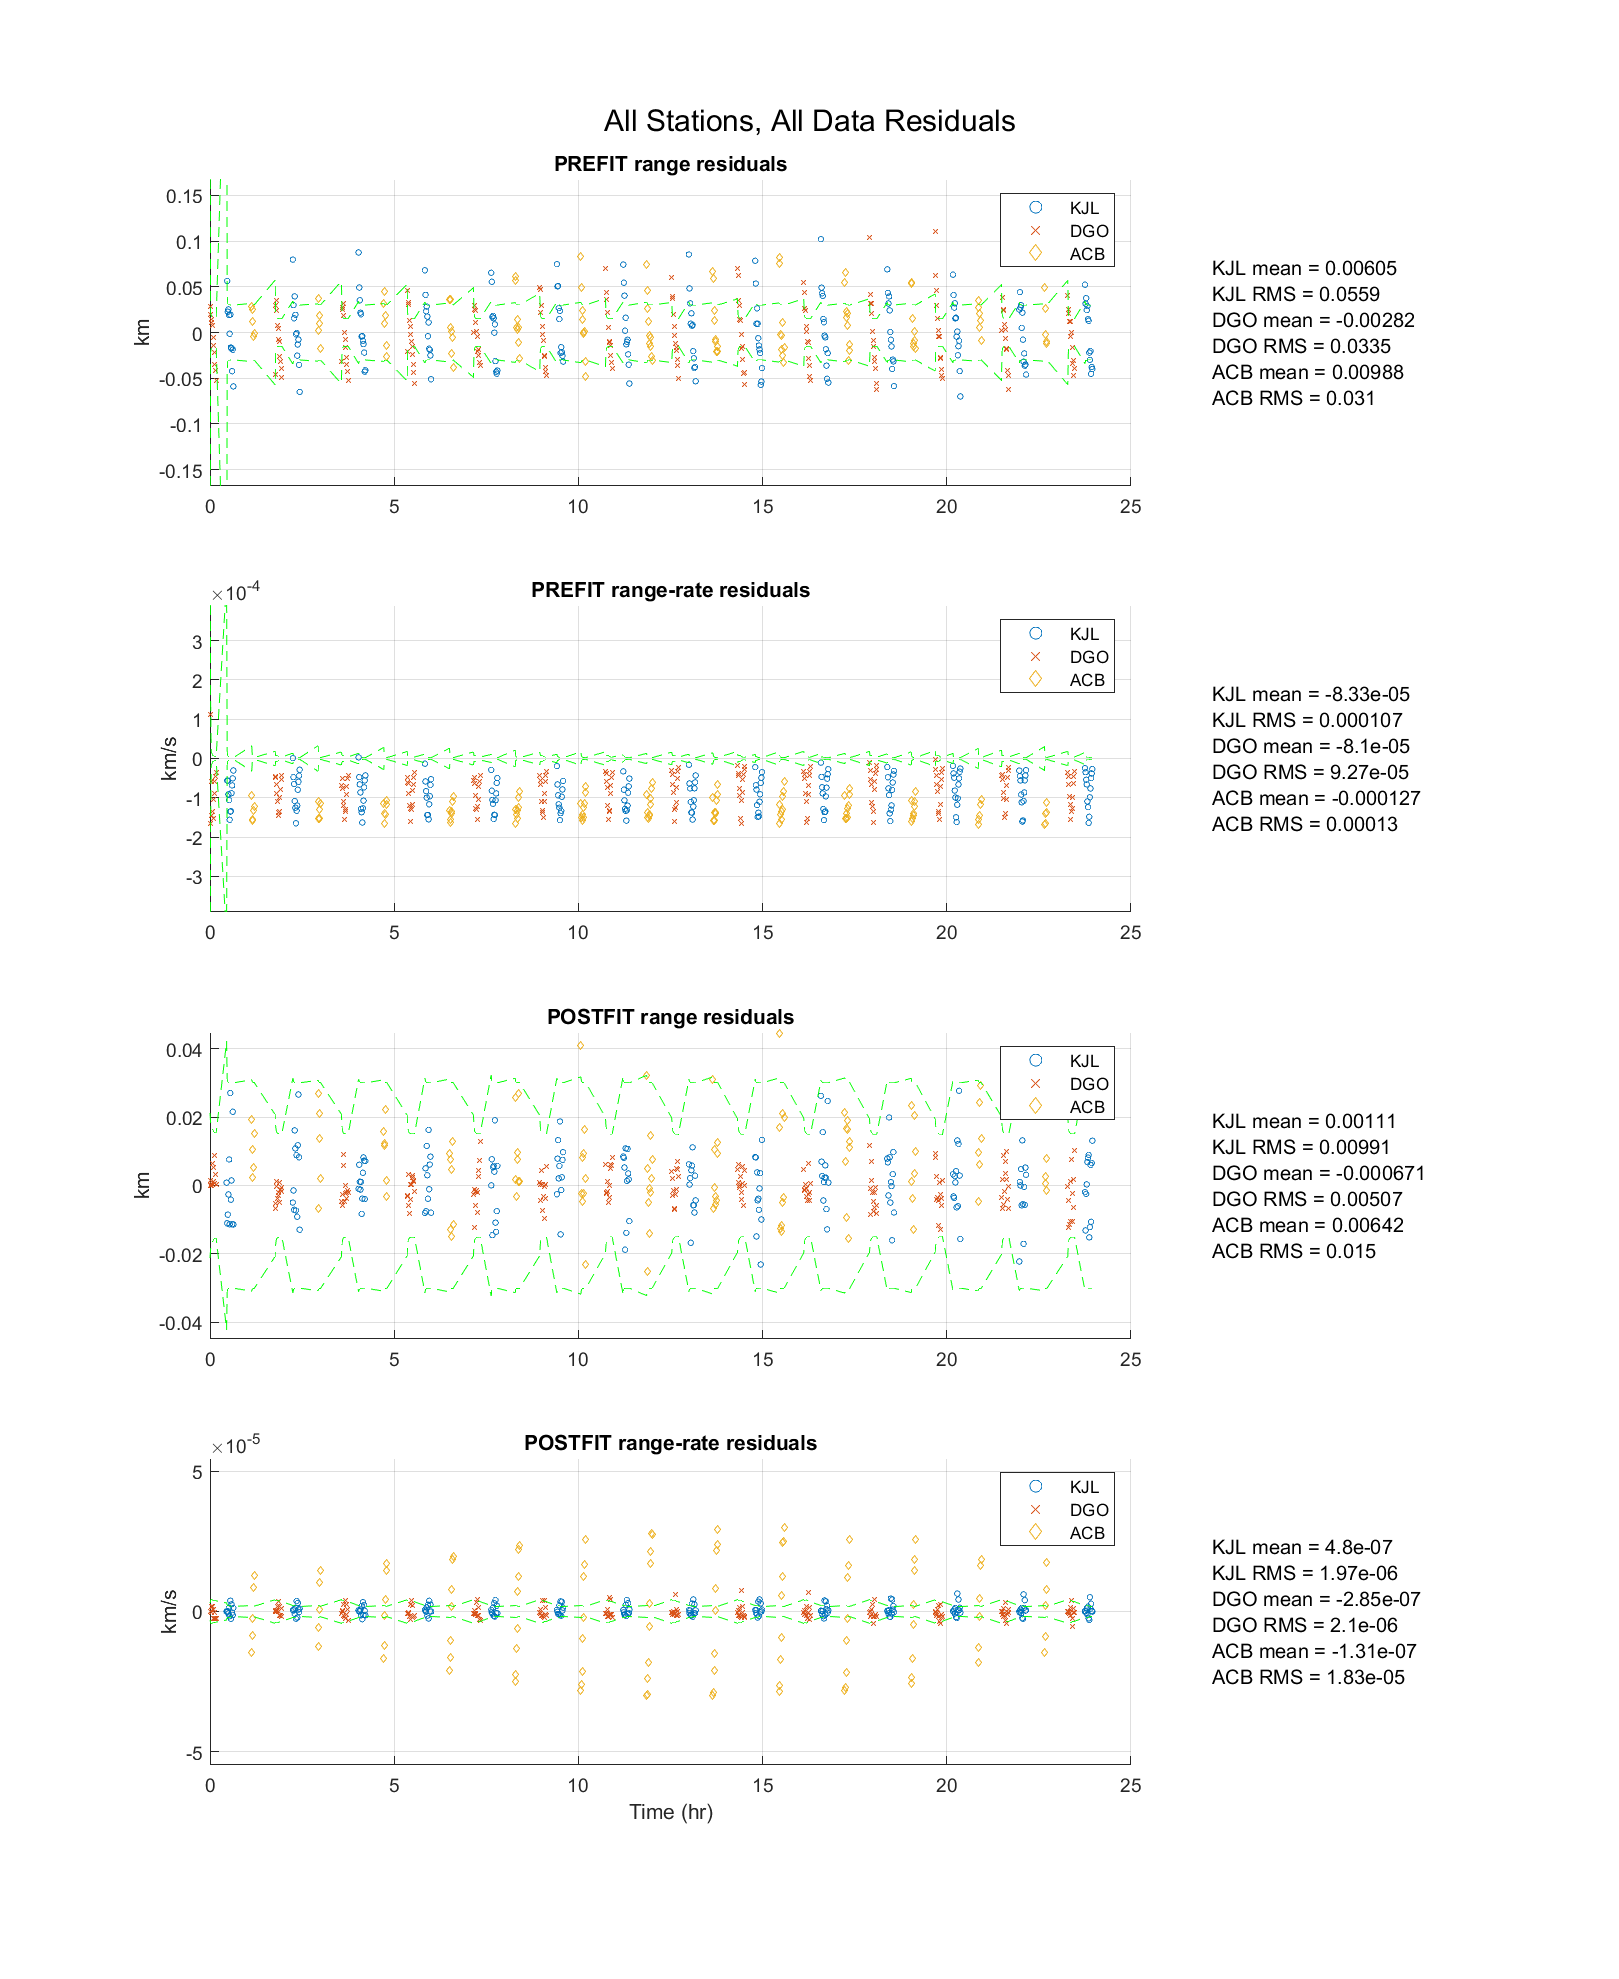
\includegraphics[width=0.8\textwidth]{yesbias.png}
\end{figure}
\label{fig:yesbias}

I was also unable to debug this phenomenon, but  I suspect that there is a bug in the measurement model which is related to the negative sign of the bias. I decided to leave the bias in the measurement model because although it made the postfit rate-rate residuals for Arecibo look worse, it improved the final delivery estimate for cases including Arecibo. 


%Provide a detailed narrative of your analyses and your interpretation of the results. What are these cases indicating to you? 

% How does each sensor and data type contribute to the overall uncertainty (knowledge and delivery)? Did you have to compensate for unmodeled dynamics? If so, how? 

% How well are you predicting future measurements? Did you infer the presence of any biases? If so, which? 

% What do you seem most sensitive to in your solutions? 

% How observable are your states and parameters? 

% What did you estimate? Did you ”consider’ any parameters? 

% Did you smooth the trajectory? If so, how did this help? 

% What was your strategy for getting your results and making it all ”work?”

%Be explicit in listing all of your assumptions as these should always caveat your analyses. Some of them follow (i.e. initial conditions, a priori uncertainty, observation model(s) used, dynamic model(s) used, spacecraft model(s) used, states and parameters estimated and/or considered, process noise model(s) used, estimation strategy used [e.g. EKF, batch, UKF, etc.]). 

% Provide a rationale for why you chose what you did and not something else, for instance. Orbit Determination and Prediction is a science and also an art with its own ”tradecraft.” Part of your evaluation is based upon this tradecraft that you developed over the course.


\section{Final thoughts} 

The range-rate data proved to be more accurate than the range data and was my best estimate. That is because range-rate also encodes some range information, in addition to range-rate data. For example, the H matrix at the first measurement was calculated as follows:  

\begin{equation}
	H_{t0} = 
	\begin{bmatrix}
		0.66516   &  -0.61572 &     0.42244    &   0 &	0  &          0 \\		      
		0.00095726  &  0.0018599  &  0.0012037   &   0.66516 &
		-0.61572    &  0.42245
	\end{bmatrix}
\end{equation}

The first row is the gradient of the range measurement with respect to the satellite position, and the second row is the gradient of the range-rate measurement with respect to the satellite position. Moreover, the standard deviation of the range data was larger than the standard deviation of the range-rate data. Kwajalein, for example, had a standard deviation of 10 m for range, but a 0.5 mm/s standard deivation for range-rate. More information and accuracy are retained in the range-rate calculation than the range calculation. Nevertheless, the range-only case was not bad, ending up 0.097 km from the best estimate. 

Kwajalein and Diego-Garcia were the most accurate stations for me. Diego-Garcia was likely the best single station for me overall, as Diego-Garcia is within 0.055 km overall of the best estimate, with Kwajalein following at 0.386 km. The final delivery Arecibo position is 0.790 km within the best case. 

I expected the short-arc case to have the best result. The state covariance was widened to 1 km in position, 1 m/s in velocity at the start of propagation, but Case G ended up as the 2nd-worst performing case at 0.763 km away from the best estimate. The long arc did not fare much better, at 0.711 km away from the best estimate. This is probably due to the inclusion of Arecibo range data. 

Dynamical errors include the drag model only accounting for solar panel. I would have liked to implement EGM2008 as well to compare with just the GRACE gravity model but was not able to in time. Rather than using SPICE, it would have been interesting to use Vallado's routine to compute the sun vector and observe the differences. The ECEF to ECI function also may have errors, likely from Earth rotation and timing, which I did not change from Homework 4. 

Overall, including as much as possible to produce finer resolution models and intelligently filtering (adjusting station covariances, process noise) would lead to better orbit determination and prediction, which is a science and, as this class has shown me, an art. 



\newpage
% ================================================================ % 
\section*{Appendix} 

\subsection*{Final Project MATLAB code} 

\textbf{Note: The equations of motion and functions to transform from ECI to ECEF and back were submitted as part of Homework 4, and so are left out of this appendix.}

\subsubsection{finalproj\_EOM\_batch.m:}
\begin{lstlisting}[basicstyle=\footnotesize]
	% HW 5 
	% Junette Hsin 
	
	% clear; clc 
	addpath(genpath('mice')); 
	addpath(genpath('spice_data')); 
	
	% Load SPICE kernel file 
	cspice_furnsh( 'spice_data/naif0011.tls' )
	cspice_furnsh( 'spice_data/de421.bsp' )       
	cspice_furnsh( 'spice_data/pck00010.tpc ') 
	
	format long g 
	
	%% Parameters 
	
	global const 
	global muE RE muS AU muM eE wE J2 J3 J4 Cd Cs eop_data 
	global A m_SC p p0 r0_drag H CD
	
	% initial state initial guess (M --> KM)
	const.CD  = 1.88;    
	% X0 = [ 6984.45711518852 
	%        1612.2547582643 
	%        13.0925904314402 
	%       -1.67667852227336
	%        7.26143715396544
	%        0.259889857225218 ]; 
	
	% ballpark right answer 
	X0  = [   6978.25613502827
	1616.30084111326
	19.7187226552466
	-1.66208631750821
	7.26104887569659
	0.270612922289392 ]; 
	
	nX  = length(X0); 
	
	% initialize STM 
	STM0 = eye(length(X0)); 
	STM0 = reshape(STM0, [length(X0)^2 1]); 
	XSTM0 = [X0; STM0];  
	
	% Constants 
	const.muE = 398600.4415;          % Earth Gravitational Parameter (km^3/s^2) 
	const.RE  = 6378.1363;            % Earth Radius (km)
	const.muS = 132712440018;         % Sun's Gravitational Parameter (km^3/s^2)
	const.AU  = 149597870.7;          % 1 Astronomical Unit (km)
	const.muM = 4902.800066;          % Moon's Gravitational Parameter (km^3/s^2)
	const.eE  = 0.081819221456;       % Earth's eccentricity 
	const.wE  = 7.292115146706979e-5; % Earth's rotational velocity (rad/s)
	const.m_SC = 2000;                 % satellite mass (kg) 
	const.Cd  = 0.04;                 % diffuse reflection 
	const.Cs  = 0.04;                 % specular reflection 
	
	% face areas 
	const.Ax = 6 / 1e6; % m^2 --> km^2 
	const.Ay = 8 / 1e6; 
	const.Az = 12 / 1e6; 
	const.Asp = 15 / 1e6; 
	
	% Cs and Cd for x, y, and z 
	const.MLI_Kapton_Cs = 0.59; 
	const.MLI_Kapton_Cd = 0.04; 
	const.White_Paint_Cs = 0.04; 
	const.White_Paint_Cd = 0.80; 
	const.Germanium_Kapton_Cs = 0.18; 
	const.Germanium_Kapton_Cd = 0.28; 
	const.Solar_Cells_Cs = 0.04; 
	const.Solar_Cells_Cd = 0.04; 
	
	const.p_srp     = 4.57e-6;     % solar pressure per unit area, in N/m^2 
	const.p_srp     = const.p_srp * 1e6; % N/m^2 --> N/km^2 
	
	const.J2 = 1.08262617385222e-3; 
	const.J3 = -2.53241051856772e-6;
	const.J4 = -1.61989759991697e-6; 
	
	global r_KJL_ECEF r_DGO_ECEF r_ACB_ECEF 
	
	% Station coords. Convert M --> KM 
	r_KJL_ECEF = [-6143584  1364250  1033743]' / 1000;  % Kwajalein 
	r_DGO_ECEF = [ 1907295  6030810 -817119 ]' / 1000;  % Diego 
	r_ACB_ECEF = [ 2390310 -5564341  1994578]' / 1000;  % Arecibo 
	
	global LEO_DATA_Apparent 
	% Load observation data 
	% load('LEO_DATA_Apparent.mat') 
	load LEO_DATA_Apparent_3Days.mat 
	test = load('LEO_DATA_Apparent_Days4-6.mat'); 
	days4to6 = test.LEO_DATA_Apparent; 
	days4to6(:,2) = days4to6(:,2) + 3*86400; 
	LEO_DATA_Apparent = [LEO_DATA_Apparent; days4to6];   
	
	% Station data 
	ID_STA   = 1; 
	i_STA    = find(LEO_DATA_Apparent(:, 1) == ID_STA); 
	Yobs_KJL = LEO_DATA_Apparent(i_STA, :); 
	t_KWJ    = Yobs_KJL(:,2); 
	
	ID_STA   = 2; 
	i_STA    = find(LEO_DATA_Apparent(:, 1) == ID_STA); 
	Yobs_DGO = LEO_DATA_Apparent(i_STA, :);
	t_DGO    = Yobs_DGO(:,2); 
	
	ID_STA   = 3; 
	i_STA    = find(LEO_DATA_Apparent(:, 1) == ID_STA); 
	Yobs_ACB = LEO_DATA_Apparent(i_STA, :);
	t_ACB    = Yobs_DGO(:,2); 
	
	eop_data = load('finals_iau1980.txt'); 
	
	% Atmospheric drag 
	r   = norm(X0(1:3));            % km 
	const.H   = 88667.0 / 1000;           % m --> km 
	const.r0_drag  = (700 + RE);          % m --> km 
	const.p0  = 3.614e-13 * 1e9;          % kg/m3 --> kg/km^3 
	const.p   = p0*exp( -(r-r0_drag)/H ); 
	const.A   = 15 / 1e6;                 % m^2 --> km^2 
	
	global Cnm Snm 
	
	% Gravity 
	Cnm = zeros(181,181);
	Snm = zeros(181,181);
	fid = fopen('GGM03S.txt','r');
	for n=0:180
	for m=0:n
	temp = fscanf(fid,'%d %d %f %f %f %f',[6 1]);        
	Cnm(n+1,m+1) = temp(3);
	Snm(n+1,m+1) = temp(4);
	end
	end
	
	%% Convert t0 to ET, i.e. seconds past J2000, the base time variable for SPICE. function calls.
	
	%  Epoch for initial conditions 
	% epoch = 23 March 2018, 08:55:03 UTC ; 
	t0      = 'March 23, 2018, 08:55:03 UTC'; 
	abcorr  = 'NONE';
	
	%  Convert the epoch to ephemeris time. 
	et_t0   = cspice_str2et( t0 );
	
	% extract observation epochs 
	epochs = LEO_DATA_Apparent(:,2); 
	epochs = et_t0 + epochs; 
	
	
	%% Derive A and H matrices 
	
	X  = sym('X', [length(X0) 1]); 
	dX = fn.EOM(et_t0, X); 
	
	% compute partials 
	Amat    = jacobian( dX, X );       
	Amat_fn = matlabFunction(Amat); 
	
	% DO EVERYTHING IN ECI FRAME 
	
	X  = sym('X', [nX; 1]); 
	XS = sym('XS', [nX; 1]); 
	
	r_site = [X(1)-XS(1); X(2)-XS(2); X(3)-XS(3)]; 
	v_site = [X(4)-XS(4); X(5)-XS(5); X(6)-XS(6)]; 
	d      = norm(r_site); 
	v      = dot(v_site, r_site/norm(r_site)); 
	
	Htmat      = sym(zeros(2,nX)); 
	Htmat(1,:) = simplify(gradient(d, X)); 
	Htmat(2,:) = simplify(gradient(v, X)); 
	Ht_fn      = matlabFunction(Htmat); 
	
	Ht_r_fn  = matlabFunction(Htmat(1,:)); 
	Ht_rr_fn = matlabFunction(Htmat(2,:)); 
	
	% Ht with G bias function 
	rbias = 0.02; 
	
	r_site = [X(1)-XS(1); X(2)-XS(2); X(3)-XS(3)]; 
	v_site = [X(4)-XS(4); X(5)-XS(5); X(6)-XS(6)]; 
	d      = norm(r_site) - rbias; 
	v      = dot(v_site, r_site / d); 
	
	Htmat      = sym(zeros(2,nX)); 
	Htmat(1,:) = simplify(gradient(d, X)); 
	Htmat(2,:) = simplify(gradient(v, X)); 
	Ht_bias_fn = matlabFunction(Htmat); 
	
	%% integrate EOM 
	
	% set ode45 params 
	rel_tol = 1e-10;         % 1e-14 accurate; 1e-6 coarse 
	abs_tol = 1e-10; 
	options = odeset('reltol', rel_tol, 'abstol', abs_tol ); 
	
	% Set run state 
	run_state = 1; 
	disp('Running sim ...') 
	
	if run_state == 1
	[t, X] = ode45(@fn.EOM, [epochs(1) : 60 : epochs(end)], X0, options); 
	elseif run_state == 2
	[t, XSTM] = ode45(@(t, XSTM) fn.EOM_STM(t, XSTM, Amat_fn, nX), [epochs(1) : 60 : epochs(end)], XSTM0, options); 
	X = XSTM(:, 1:6); 
	end 
	disp('Pos and Vel end: ')
	disp(X(end, 1:6)'); 
	
	XSTM_ref0   = XSTM; 
	t_XSTM_ref0 = t; 
	
	
	%% Setting up filters 
	
	% weighting matrices m --> km, mm --> km 
	global R_KJL R_DGO R_ACB 
	const.R_KJL = [(10e-3)^2 0; 0 (0.5e-6)^2]; 
	const.R_DGO = [(5e-3)^2  0; 0 (1e-6)^2]; 
	const.R_ACB = [(10e-3)^2 0; 0 (0.5e-6)^2]; 
	
	% initial covariance error 
	% 10 km std - position 
	% 10 m/s    - velocity 
	P0 = [ 10^2*eye(3), zeros(3); 
	zeros(3),  (10e-3)^2*eye(3) ]; 
	Lambda0 = inv(P0); 
	global Lambda_KJL0 Lambda_DGO0 Lambda_ACB0
	Lambda_KJL0 = Lambda0; 
	Lambda_DGO0 = Lambda0; 
	Lambda_ACB0 = Lambda0; 
	
	global N_KJL0 N_DGO0 N_ACB0
	N0    = Lambda0*X0; 
	N_KJL0 = N0; 
	N_DGO0 = N0; 
	N_ACB0 = N0; 
	
	
	%% Batch all stations to refine IC 
	
	Xstar  = 100*ones(1,3); 
	XSTM   = XSTM_ref0; 
	t_XSTM = t_XSTM_ref0; 
	XSTM0  = XSTM_ref0(1,:)'; 
	iter   = 0; 
	N_prev = N0; 
	Lambda_prev = Lambda0; 
	
	% Batch first 28 measurements 
	
	tic 
	while norm(Xstar(1:3)) > 0.1
	
	% keep track of iterations 
	iter = iter + 1; 
	sprintf('iter = %d', iter)
	
	% Test - All stations 
	[Ycalc_all, Lambda, N] = ... 
	fn.batch_LSQ(LEO_DATA_Apparent, t_XSTM, XSTM, et_t0, Ht_fn, Lambda_prev, N_prev); 
	
	%     % Test - Kwajalein 
	%     [Ycalc_all, Lambda, N] = ... 
	%         fn.batch_LSQ(Yobs_KJL, t_XSTM, XSTM, et_t0, Ht_fn, Lambda0, N0); 
	
	% Solve normal equation 
	Xstar = inv(Lambda) * N; 
	
	% update covariance 
	Lambda_prev = Lambda0; 
	N_prev      = N0; 
	
	% update initial conditions 
	XSTM0(1:nX) = XSTM0(1:nX) + Xstar; 
	[t, XSTM] = ode45(@(t, XSTM) fn.EOM_STM(t, XSTM, Amat_fn, nX), [epochs(1) : 60 : epochs(end)], XSTM0, options); 
	
	disp('xhat pos'); Xstar(1:3)
	disp('xhat pos norm'); norm(Xstar(1:3))
	disp('x IC pos'); XSTM0(1:3)
	
	end 
	toc 
	
	Lambda_batch = Lambda; 
	XSTM_batch   = XSTM; 
	XSTM0_batch  = XSTM0; 
	
	
\end{lstlisting}

\subsubsection{finalproj\_EKF.m:}
\begin{lstlisting}


% HW 5 
% Junette Hsin 

% finalproj_EOM_batch; 
close all; format long g; 
load WS_batch.mat 

% Load SPICE stuff 
addpath(genpath('mice')); 
addpath(genpath('spice_data')); 
cspice_furnsh( 'spice_data/naif0011.tls' )
cspice_furnsh( 'spice_data/de421.bsp' )       
cspice_furnsh( 'spice_data/pck00010.tpc ' ) 

%% 

global eopdata const

SAT_Const

% read Earth orientation parameters
fid = fopen('eop19620101.txt','r');
%  ----------------------------------------------------------------------------------------------------
% |  Date    MJD      x         y       UT1-UTC      LOD       dPsi    dEpsilon     dX        dY    DAT
% |(0h UTC)           "         "          s          s          "        "          "         "     s 
%  ----------------------------------------------------------------------------------------------------
eopdata = fscanf(fid,'%i %d %d %i %f %f %f %f %f %f %f %f %i',[13 inf]);
fclose(fid);

%%

% plot options 
plot_orbit = 0; 
plot_RSW   = 0; 

% Selct sim params 
run_STA  = 1 ;      % run STATIONS 
run_DATA = 0 ;      % run DATA 
save_nag = 0 ;      % save NAG 
DAYS     = 1;       % PROPAGATE to 1 day, 3 days, or 7 days. 

%% EKF - all observations 

% loop through STATIONS 
if run_STA == 1
DATA = 0;       % 0 = all data 
for STATIONS = 3    % 0 = all stations, 1 = KJL, 2 = DGO, 3 = ACB
EKF_STA_DATA; 
end
end 

% loop through DATA 
if run_DATA == 1
STATIONS = 0;       % 0 = all stations 
for DATA = 1:2      % 0 = all data, 1 = range, 2 = range-rate, 3 = short-arc 
EKF_STA_DATA; 
end
end

X_sol1 = [ -6330.16736001325
3306.81591178162
127.736863438565
-3.43787907681733
-6.63350511630163
-0.235613730204275 ]; 


%% save NAG 

% Save in NAG format 
if save_nag == 1

load WS_R_7.mat     % case A 
save_case(Xi, P_bar, 'A'); 
load WS_RR_7.mat    % case B 
save_case(Xi, P_bar, 'B'); 
load WS_KJL_7.mat   % case C 
save_case(Xi, P_bar, 'C'); 
load WS_DGO_7.mat   % case D 
save_case(Xi, P_bar, 'D'); 
load WS_ACB_7.mat   % case E 
save_case(Xi, P_bar, 'E'); 
load WS_ALL_7.mat   % case F (LONG arc now) 
save_case(Xi, P_bar, 'F'); 
load WS_ALL_7_short_arc.mat   % case F (short arc now) 
save_case(Xi, P_bar, 'G'); 

save('hsinj.mat' ... 
, 'hsinj_pos_caseA', 'hsinj_poscov_caseA' ...   % Range only 
, 'hsinj_pos_caseB', 'hsinj_poscov_caseB' ...   % Range-rate only 
, 'hsinj_pos_caseC', 'hsinj_poscov_caseC' ...   % Kwajalein only 
, 'hsinj_pos_caseD', 'hsinj_poscov_caseD' ...   % Diego-Garcia only 
, 'hsinj_pos_caseE', 'hsinj_poscov_caseE' ...   % Arecibo only 
, 'hsinj_pos_caseF', 'hsinj_poscov_caseF' ...   % All stations, all data 
, 'hsinj_pos_caseG', 'hsinj_poscov_caseG' ... 
);  

end

%% subfunctions 

function save_case(Xi, P_bar, case_str)

pos_str = ['hsinj_pos_case' case_str]; 
poscov_str = ['hsinj_poscov_case' case_str]; 

evalin('base', [pos_str, ' = Xi(1:3)'])     % Not recommended but oh well 
evalin('base', [poscov_str, ' = P_bar(1:3,1:3)'])     % Not recommended but oh well 

end


\end{lstlisting}

\textbf{batch\_LSQ.m:}
\begin{lstlisting}
function [Ycalc_STA, Lambda, N] = ... 
batch_LSQ(Yobs_STA, t_XSTM, XSTM, et_t0, Ht_fn, Lambda0, N0)

global wE R_KJL R_DGO R_ACB 
global r_KJL_ECEF r_DGO_ECEF r_ACB_ECEF 

% Initialize calculated Y 
Ycalc_STA = zeros(size(Yobs_STA)); 
Ycalc_STA(:, 1:2) = Yobs_STA(:, 1:2); 

% Set up covariance 
nX     = length(N0); 
Lambda = Lambda0; 
N      = N0; 

% for i = 1:length(Yobs_STA)
for i = 1:28

% find index for same time state and observation 
Yi   = Yobs_STA(i, :); 
ti   = Yi(2) + et_t0; 
i_X  = find(t_XSTM == ti); 

% get JD time 
JD_UTC = cspice_et2utc(ti, 'J', 10); 
JD_UTC = str2num(extractAfter(JD_UTC, 'JD ')); 

% observation covariance 
if Yi(1) == 1
R = R_KJL; 
r_STA_ECEF = r_KJL_ECEF; 
elseif Yi(1) == 2
R = R_DGO; 
r_STA_ECEF = r_DGO_ECEF; 
else 
R = R_ACB; 
r_STA_ECEF = r_ACB_ECEF; 
end 

% Convert station to ECI frame 
r_STA_ECI  = fn.ECEFtoECI(JD_UTC, r_STA_ECEF); 
v_KJL_ECEF = [0; 0; 0]; 
a_ECEF     = v_KJL_ECEF + cross([ 0 0 wE ]', r_STA_ECEF); 
v_STA_ECI  = fn.ECEFtoECI(JD_UTC, a_ECEF); % Technically wrong. Look in Vallado 
XSi        = [r_STA_ECI; v_STA_ECI]; 

% Extract states (all in ECI) 
Xi   = XSTM( i_X, 1:nX)'; 
STMi = XSTM( i_X, nX+1 : nX+nX^2 ); 
STMi = reshape(STMi, [nX nX]); 

% compute H [2x7]
Hi = Ht_fn(Xi(1), Xi(2), Xi(3), Xi(4), Xi(5), Xi(6), XSi(1), XSi(2), XSi(3), XSi(4), XSi(5), XSi(6)) * STMi; 

% Accumulate observation 
Ycalc_STA(i,3:4) = Hi * Xi; 

% Obtain y difference 
yi = Yobs_STA(i,3:4)' - fn.G_fn(Xi, XSi); 

% Accumulate covariance 
Lambda = Lambda + Hi' * inv(R) * Hi; 
N      = N + Hi' * inv(R) * yi; 

end 

end 
\end{lstlisting}

\subsubsection{EKF\_STA\_DATA.m}

\begin{lstlisting}
	% HW 5 
	% Junette Hsin 
	% TEST EKF SCRIPT 
	
	% weighting matrices m --> km, mm --> km 
	global R_KJL R_DGO R_ACB 
	R_KJL = [(10e-3)^2 0; 0 (0.5e-6)^2]; 
	R_DGO = [(5e-3)^2  0; 0 (1e-6)^2]; 
	R_ACB = [(10e-3)^2 0; 0 (0.5e-6)^2]; 
	
	% try smaller P0 
	P_prev     = [ diag([0.1 0.1 0.1]).^2, zeros(3); zeros(3), diag([0.1e-3 0.1e-3 0.1e-3]).^2 ]; 
	
	if DAYS == 1        % 1 day 
	load LEO_DATA_Apparent.mat 
	hrs = 24 * 1; 
	elseif DAYS == 3    % 3 days 
	load('LEO_DATA_Apparent_3Days.mat')    
	hrs = 24 * 7; 
	else                % 7 days 
	load LEO_DATA_Apparent_3Days.mat 
	temp = load('LEO_DATA_Apparent_Days4-6.mat'); 
	days4to6 = temp.LEO_DATA_Apparent; 
	days4to6(:,2) = days4to6(:,2) + 3*86400; 
	LEO_DATA_Apparent = [LEO_DATA_Apparent; days4to6];   
	hrs = 24 * 7; 
	end
	
	Yobs_STA   = LEO_DATA_Apparent;
	et_obs     = Yobs_STA(:,2) + et_t0; 
	XSTM_prev  = XSTM0_batch; 
	iter       = 0; 
	
	% SHORT ARC 
	if DATA == 3
	
	load WS_ALL_3.mat
	
	temp = load('LEO_DATA_Apparent_Days4-6.mat'); 
	days4to6 = temp.LEO_DATA_Apparent; 
	days4to6(:,2) = days4to6(:,2) + 3*86400; 
	LEO_DATA_Apparent = days4to6; 
	% propagate to last day, which is now the 4th day. hrs = 24*4 = 96 
	hrs = 24*4;  
	
	% try smaller P0 ... but wider than other cases for short arc 
	P_prev     = [ diag([1 1 1]).^2, zeros(3); zeros(3), diag([1e-3 1e-3 1e-3]).^2 ]; 
	
	X_EKF0     = X_EKF(end,:)'; 
	XSTM_prev  = [X_EKF0; STM0];
	t_EKF0     = t_X_EKF(end); 
	et_t0      = t_EKF0; 
	end
	
	if STATIONS == 0    % use all station data 
	elseif STATIONS == 1 % Kwajalein 
	R_DGO = R_DGO * 1e10; 
	R_ACB = R_ACB * 1e10; 
	elseif STATIONS == 2 % Diego 
	R_KJL = R_KJL * 1e10; 
	R_ACB = R_ACB * 1e10; 
	elseif STATIONS == 3 % STATIONS == 3 % Arecibo
	R_KJL = R_KJL * 1e10; 
	R_DGO = R_DGO * 1e10; 
	elseif STATIONS == 4 % Kwajalein and Diego - NO ARECIBO 
	R_ACB = R_ACB * 1e10; 
	elseif STATIONS == 5 % Kwajalein and Arecibo - NO DIEGO 
	R_DGO = R_DGO * 1e10; 
	else % STATIONS == 6. Diego and Arecibo - NO KWAJALEIN 
	R_KJL = R_KJL * 1e10; 
	end
	
	X_EKF      = [];     t_X_EKF    = [];     Y_prefit   = [];     Y_postfit  = []; 
	Lpre_mat   = [];     Lpost_mat  = [];     sigma3_pre = [];     sigma3_post = []; 
	
	% EKF 
	tic
	for i = 1:length(et_obs) 
	
	% keep track of iterations 
	iter = iter + 1; 
	sprintf('iter = %d', iter)
	
	% Propagate state 
	if     i == 1 && et_obs(1) == et_t0; t_prop = et_obs(i); 
	elseif i == 1;                       t_prop = [et_t0 : 60 : et_obs(1) ]; 
	else                                
	%         t_prop = [et_obs(i-1) : 60 : et_obs(i)]; 
	t_prop = [t_lt et_obs(i)]; 
	end
	
	% EKF. All data, range, or range-only 
	[t_XSTM, XSTM, Xstar, Y_pre, Y_post, P, L_pre, L_post, t_lt] = fn.EKF(Yobs_STA, XSTM_prev, nX, ... 
	epochs(1), t_prop, options, Amat_fn, Ht_fn, Ht_bias_fn, Ht_r_fn, Ht_rr_fn, P_prev, DATA); 
	
	% save states from current iteration 
	if i == 1 && et_obs(1) == et_t0; X_EKF = XSTM(1:nX)'; 
	else;                            X_EKF = [X_EKF; XSTM(:, 1:nX)]; 
	end 
	
	t_X_EKF   = [t_X_EKF; t_XSTM]; 
	Y_prefit  = [Y_prefit; Y_pre]; 
	Y_postfit = [Y_postfit; Y_post]; 
	
	% update measurement for next iteration 
	XSTM_prev = [Xstar; STM0]; 
	P_prev    = P;
	
	% innovations covariance 
	Lpre_mat  = [Lpre_mat; L_pre]; 
	Lpost_mat = [Lpost_mat; L_post]; 
	
	% 3-sigma STD 
	if DATA == 0
	sigma3_pre  = [sigma3_pre; sqrt(L_pre(1,1))*3, sqrt(L_pre(2,2))*3];  
	sigma3_post = [sigma3_post; sqrt(L_post(1,1))*3, sqrt(L_post(2,2))*3];  
	else  
	sigma3_pre  = [sigma3_pre; sqrt(L_pre(1,1))*3];  
	sigma3_post = [sigma3_post; sqrt(L_post(1,1))*3];  
	end
	
	end 
	toc
	
	%% Propagate to last period of time 
	
	t_prop = [ et_obs(end) : 60 : et_t0 + 60*60*hrs ]; 
	[t_XSTM, XSTM] = ode45(@(t, XSTM) fn.EOM_STM(t, XSTM, Amat_fn, nX), t_prop, XSTM_prev, options); 
	Xi   = XSTM(end,1:nX)'; 
	STMi = XSTM(end,nX+1:end); 
	STMi = reshape(STMi, [nX nX]); 
	
	T_ECI2RSW = fn.ECItoRSW_T(Xi); 
	T_RSW2ECI = T_ECI2RSW';
	
	% Time update + process noise 
	% dt       = t_prop(end) - t_prop(1); 
	dt       = 60; 
	Q        = diag( (100e-10)^2 * [1 1 1] ); 
	Gamma    = [diag( dt^2/2 * [1 1 1] ); diag([dt dt dt])]; 
	P_noise  = Gamma * Q * Gamma'; 
	
	RSW_Q    = diag( [1e-10^2 1000e-10^2 1e-10^2] ); 
	RSW_noise = Gamma * RSW_Q * Gamma'; 
	
	P_bar    = STMi * P_prev * STMi' + P_noise +  RSW_noise; 
	
	% Save propagated states 
	X_prop   = XSTM(:,1:nX); 
	t_X_prop = t_XSTM; 
	
	% PLOT RESIDUALS 
	EKF_res; 
	
	%% Save data 
	
	if STATIONS == 0        % all stations 
	if DATA == 0        % all data 
	ws_mat         = 'WS_ALL';  
	elseif DATA == 1    % range only 
	ws_mat         = 'WS_R';    
	elseif DATA == 2    % range-rate only 
	ws_mat         = 'WS_RR';   
	else                % DATA == 3, short arc 
	ws_mat         = 'WS_ALL_short'; 
	end
	elseif STATIONS == 1    % Kwajalein only 
	ws_mat             = 'WS_KJL';  
	elseif STATIONS == 2    % Diego-Gardcia only 
	ws_mat             = 'WS_DGO';  
	elseif STATIONS == 3    % Arecibo only 
	ws_mat             = 'WS_ACB';  
	elseif STATIONS == 4;   ws_mat = 'WS_KJL_DGO';
	elseif STATIONS == 5;   ws_mat = 'WS_KJL_ACB'; 
	else;                   ws_mat = 'WS_DGO_ACB'; % STATIONS == 6
	end 
	
	if DAYS == 1;           ws_mat = [ ws_mat '_1.mat' ];   % DAYS = 1
	elseif DAYS == 3;       ws_mat = [ ws_mat '_3.mat' ];   % DAYS = 3
	else;                   ws_mat = [ ws_mat '_7.mat' ];   % DAYS = 7
	end
	
	save(ws_mat); 
	
	
	%% radial-intrack-cross-track frame transformation for best estimate 
	plot_RSW = 1; 
	if plot_RSW == 1
	
	% RANGE-RATE         
	X_best = [ 445.715135753907
	-7100.16248363109
	-183.851374717676
	7.48601245362928
	0.469793893676187
	0.177543134574878 ]; 
	
	T_best = fn.ECItoRSW_T(X_best); 
	
	dr_ECI = X_best(1:3) - Xi(1:3); 
	
	% transform all measurements 
	dr_RSW = T_best * dr_ECI; 
	
	% Plot radial-intrack-crosstrack 
	%     ftitle = 'Radial-Intrack-Crosstrack'; 
	RICtitle = strrep(ftitle, 'Residuals', 'RIC Error'); 
	figh = figure('name', ftitle, 'position', [100 100 600 800]); 
	subplot(3,1,1)
	scatter(dr_RSW(1), dr_RSW(2)); hold on; 
	P = P_bar(1:2, 1:2); 
	h3 = fn.plot_gaussian_ellipsoid([dr_RSW(1) dr_RSW(2)], P); 
	xlabel('R (km)')
	ylabel('S (km)')
	title('Radial-Intrack') 
	subplot(3,1,2) 
	scatter(dr_RSW(1), dr_RSW(3)); hold on; 
	P = [P_bar(1), P_bar(1,3); P_bar(3,1), P_bar(3,3)]; 
	h3 = fn.plot_gaussian_ellipsoid([dr_RSW(1) dr_RSW(3)], P); 
	xlabel('R (km)')
	ylabel('W (km)')
	title('Radial-Crosstrack') 
	subplot(3,1,3) 
	scatter(dr_RSW(2), dr_RSW(3)); hold on; 
	P = P_bar(2:3, 2:3); 
	h3 = fn.plot_gaussian_ellipsoid([dr_RSW(2) dr_RSW(3)], P); 
	xlabel('S (km)')
	ylabel('W (km)')
	title('Intrack-Crosstrack')
	
	sgtitle(RICtitle); 
	
	% Vallado ed 4 p. 229 
	end
	
	
	%% Plot satellite position 
	
	if plot_orbit == 1
	ftitle = 'JahSat Orbit'; 
	figure('name', ftitle); 
	plot3(XSTM_ref0(:,1), XSTM_ref0(:,2), XSTM_ref0(:,3)); hold on; grid on; 
	plot3(XSTM_batch(:,1), XSTM_batch(:,2), XSTM_batch(:,3)); 
	plot3(X_EKF(:,1), X_EKF(:,2), X_EKF(:,3));  
	plot3(X_prop(:,1), X_prop(:,2), X_prop(:,3))
	xlabel('x (km)'); ylabel('y (km)'); zlabel('z (km)'); 
	legend('initial', 'batch', 'EKF', 'prop') 
	title(ftitle)
	end
	
\end{lstlisting}

\textbf{EKF.m:}
\begin{lstlisting}
	function [t_XSTM, XSTM, X_update, Y_prefit, Y_postfit, P_update, L_pre, L_post, t_lt] = ... 
	EKF(Yobs_STA, XSTM_prev, nX, et_t0, t_prop, options, Amat_fn, Ht_fn, Ht_bias_fn, Ht_r_fn, Ht_rr_fn, P_prev, DATA)
	
	global R_KJL R_DGO R_ACB 
	global r_KJL_ECEF r_DGO_ECEF r_ACB_ECEF 
	
	% Integrate ref trajectory and STM from t = i-1 (prev) to t = i (curr) 
	if length(t_prop) > 1
	[t_XSTM, XSTM] = ode45(@(t, XSTM) fn.EOM_STM(t, XSTM, Amat_fn, nX), t_prop, XSTM_prev, options); 
	Xi   = XSTM(end,1:nX)'; 
	STMi = XSTM(end,nX+1:end); 
	else
	t_XSTM = t_prop; 
	XSTM = XSTM_prev; 
	Xi   = XSTM(1:nX); 
	STMi = XSTM(nX+1:end); 
	end 
	STMi = reshape(STMi, [nX nX]); 
	
	% find index for same time state and observation 
	t_Y   = Yobs_STA(:,2) + et_t0; % time after initial epoch 
	ti_X  = t_XSTM(end); 
	i_Y   = find(t_Y == ti_X); 
	Yi    = Yobs_STA(i_Y, :); 
	
	% observation covariance 
	if Yi(1) == 1 
	R = R_KJL; 
	r_STA_ECEF = r_KJL_ECEF; 
	elseif Yi(1) == 2 
	R = R_DGO; 
	r_STA_ECEF = r_DGO_ECEF; 
	else 
	R = R_ACB; 
	r_STA_ECEF = r_ACB_ECEF; 
	end 
	
	% get JD time 
	JD_UTC = cspice_et2utc(t_XSTM(end), 'J', 10); 
	JD_UTC = str2num(extractAfter(JD_UTC, 'JD ')); 
	
	% Convert station to ECI frame 
	XSi_OG = rv_ECEFtoECI(JD_UTC, r_STA_ECEF, [0; 0; 0]); 
	MJD_UTC = JD_UTC - 2400000.5; 
	XSi = ECEF2ECI( MJD_UTC, [r_STA_ECEF; 0; 0; 0] ); 
	
	% Time update + process noise 
	dt    = t_prop(end) - t_prop(1); 
	Q     = diag( (10e-10)^2 * [1 1 1] ); 
	Gamma = [diag( dt^2/2 * [1 1 1] ); diag([dt dt dt])]; 
	P_noise = Gamma * Q * Gamma'; 
	Ppre_bar = STMi * P_prev * STMi' + P_noise; 
	
	% Y prefit 
	Y_prefit(1:2) = Yi(1:2); 
	Y_prefit(3:4) = fn.G_fn(Xi, XSi)'; 
	
	% PREFIT Observation-state matrix 
	if DATA == 0 || DATA == 3
	Hti_pre = Ht_fn(Xi(1), Xi(2), Xi(3), Xi(4), Xi(5), Xi(6), XSi(1), XSi(2), XSi(3), XSi(4), XSi(5), XSi(6)); 
	elseif DATA == 1
	R = R(1,1); 
	Hti_pre = Ht_r_fn(Xi(1), Xi(2), Xi(3), XSi(1), XSi(2), XSi(3)); 
	else % DATA == 2
	R = R(2,2); 
	Hti_pre = Ht_rr_fn(Xi(1), Xi(2), Xi(3), Xi(4), Xi(5), Xi(6), XSi(1), XSi(2), XSi(3), XSi(4), XSi(5), XSi(6)); 
	end
	
	% PREFIT Innovation (information) covariance 
	L_pre = (Hti_pre * Ppre_bar * Hti_pre' + R); 
	
	% CORRECT + UPDATE. Light time correction 
	c     = 299792.458; % km/s 
	lt    = Y_prefit(3) / c;  % range / c = delta time (s) 
	t_lt  = ti_X - lt; 
	t_back = [ti_X, t_lt];  
	if length(t_prop) > 1 
	XSTM_end = XSTM(end,:); 
	else
	XSTM_end = XSTM; 
	end
	nX = length(Xi); 
	[~, XSTM_lt] = ode45(@(t, XSTM) fn.EOM_STM(t, XSTM, Amat_fn, nX), t_back, XSTM_end, options); 
	Xi_lt        = XSTM_lt(end,1:nX)'; 
	
	% Satellite ECI coords with aberration and light time corrections. IF
	% RANGE-RATE ONLY, TURN OFF ABERRATION 
	v_STA_ECI      = XSi(4:6); 
	Xi_lt_abr      = Xi_lt; 
	% if ~isequal(DATA, 2)
	%     Xi_lt_abr(1:3) = Xi_lt(1:3) + lt * v_STA_ECI; 
	% end 
	
	if DATA == 0 || DATA == 3
	
	% Compute Hti again, with satellite ECI lt and abr corrected state, and same station ECI state 
	Hti_lt_abr = Ht_bias_fn(Xi_lt_abr(1), Xi_lt_abr(2), Xi_lt_abr(3), Xi_lt_abr(4), Xi_lt_abr(5), Xi(6), ... 
	XSi(1), XSi(2), XSi(3), XSi(4), XSi(5), XSi(6)); 
	%     Hti_lt_abr = Ht_fn(Xi_lt_abr(1), Xi_lt_abr(2), Xi_lt_abr(3), Xi_lt_abr(4), Xi_lt_abr(5), Xi(6), ... 
	%         XSi(1), XSi(2), XSi(3), XSi(4), XSi(5), XSi(6)); 
	
	% Gain matrix 
	Ki = Ppre_bar * Hti_lt_abr' * inv( Hti_lt_abr * Ppre_bar * Hti_lt_abr' + R ); 
	
	% Obtain y difference 
	yi = Yi(3:4)' - fn.G_bias_fn(Xi_lt_abr, XSi, Yi(1)); 
	%     yi = Yi(3:4)' - fn.G_fn(Xi_lt_abr, XSi); 
	%     yi(1) = yi(1) + rbias; 
	
	elseif DATA == 1
	
	% Compute Hti again, with satellite ECI lt and abr corrected state, and same station ECI state 
	Hti_lt_abr = Ht_r_fn(Xi_lt_abr(1), Xi_lt_abr(2), Xi_lt_abr(3), XSi(1), XSi(2), XSi(3)); 
	
	% Gain matrix 
	Ki = Ppre_bar * Hti_lt_abr' * inv( Hti_lt_abr * Ppre_bar * Hti_lt_abr' + R); 
	
	% Obtain y difference (range only) 
	yi = Yi(3:4)' - fn.G_fn(Xi_lt_abr, XSi); 
	%     yi = Yi(3:4)' - fn.G_bias_fn(Xi_lt_abr, XSi, Yi(2)); 
	yi = yi(1); 
	
	elseif DATA == 2
	
	% Compute Hti again, with satellite ECI lt and abr corrected state, and same station ECI state 
	Hti_lt_abr = Ht_rr_fn(Xi_lt_abr(1), Xi_lt_abr(2), Xi_lt_abr(3), Xi_lt_abr(4), Xi_lt_abr(5), Xi_lt_abr(6), ... 
	XSi(1), XSi(2), XSi(3), XSi(4), XSi(5), XSi(6)); 
	
	% Gain matrix 
	Ki = Ppre_bar * Hti_lt_abr' * inv( Hti_lt_abr * Ppre_bar * Hti_lt_abr' + R); 
	
	% Obtain y difference (range-rate only) 
	yi = Yi(3:4)' - fn.G_fn(Xi_lt_abr, XSi); 
	yi = yi(2); 
	
	end
	
	% Measurement and reference orbit update. Add xhat to dynamically propagated satellite ECI state  
	xhat     = Ki * yi; 
	if norm(xhat(1:3)) > 50 
	disp('xhat pos > 50'); return 
	end
	X_update = Xi_lt + xhat; 
	nX       = length(Xi); 
	P_update = ( eye(nX) - Ki * Hti_pre ) * Ppre_bar; 
	
	% POSTFIT Observation-state matrix <-- FIX, USE XSi 
	if DATA == 0 || DATA == 3
	Hti_post = Ht_fn(X_update(1), X_update(2), X_update(3), X_update(4), X_update(5), X_update(6), ... 
	XSi(1), XSi(2), XSi(3), XSi(4), XSi(5), XSi(6)); 
	elseif DATA == 1
	Hti_post = Ht_r_fn(X_update(1), X_update(2), X_update(3), XSi(1), XSi(2), XSi(3)); 
	else
	Hti_post = Ht_rr_fn(X_update(1), X_update(2), X_update(3), X_update(4), X_update(5), X_update(6), ... 
	XSi(1), XSi(2), XSi(3), XSi(4), XSi(5), XSi(6));     
	end
	
	% POSTFIT Innovation (information) covariance 
	
	L_post = (Hti_post * P_update * Hti_post' + R); 
	
	% Y postfit 
	Y_postfit(1:2) = Yi(1:2); 
	Y_postfit(3:4) = fn.G_fn(X_update, XSi)'; 
	
	
	end 
	
	%% subfunctions 
	
	function XSi = rv_ECEFtoECI(JD_UTC, r_STA_ECEF, v_STA_ECEF)
	
	global wE 
	
	r_STA_ECI  = fn.ECEFtoECI(JD_UTC, r_STA_ECEF); 
	v_STA_ECI  = v_STA_ECEF + cross([ 0 0 wE ]', r_STA_ECEF); 
	v_STA_ECI  = fn.ECEFtoECI(JD_UTC, v_STA_ECI); % Technically wrong. Look in Vallado p. 228 
	XSi        = [r_STA_ECI; v_STA_ECI]; 
	
	end

\end{lstlisting}

\subsubsection{EKF\_res.m}
\begin{lstlisting}
	
	
	
	%% Calculate residuals 
	
	Ypre_KJL   = [];    Ypre_DGO   = [];    Ypre_ACB   = []; 
	Ypost_KJL  = [];    Ypost_DGO  = [];    Ypost_ACB  = []; 
	sigma3_KJL = [];    sigma3_DGO = [];    sigma3_ACB = []; 
	
	% Extract states that correspond with station measurements 
	for i = 1:length(Y_postfit)
	
	ti  = Y_postfit(i, 2); 
	ti  = ti + et_t0; 
	i_X = find(t_X_EKF == ti); 
	i_STA = Y_postfit(i, 1); 
	
	if i_STA == 1
	Ypre_KJL   = [Ypre_KJL; Y_prefit(i,:)]; 
	Ypost_KJL  = [Ypost_KJL; Y_postfit(i,:)];  
	elseif i_STA == 2
	Ypre_DGO   = [Ypre_DGO; Y_prefit(i,:)]; 
	Ypost_DGO  = [Ypost_DGO; Y_postfit(i,:)];  
	else
	Ypre_ACB   = [Ypre_ACB; Y_prefit(i,:)]; 
	Ypost_ACB  = [Ypost_ACB; Y_postfit(i,:)];  
	end 
	
	end 
	
	
	% Station data 
	i_STA    = find(LEO_DATA_Apparent(:, 1) == 1); 
	Yobs_KJL = LEO_DATA_Apparent(i_STA, :); 
	i_STA    = find(LEO_DATA_Apparent(:, 1) == 2); 
	Yobs_DGO = LEO_DATA_Apparent(i_STA, :);
	i_STA    = find(LEO_DATA_Apparent(:, 1) == 3); 
	Yobs_ACB = LEO_DATA_Apparent(i_STA, :);
	[dpre_err_KJL, dpre_rms_KJL, vpre_err_KJL, vpre_rms_KJL] = calc_res_all(Yobs_KJL, Ypre_KJL, DATA); 
	[dpre_err_DGO, dpre_rms_DGO, vpre_err_DGO, vpre_rms_DGO] = calc_res_all(Yobs_DGO, Ypre_DGO, DATA); 
	[dpre_err_ACB, dpre_rms_ACB, vpre_err_ACB, vpre_rms_ACB] = calc_res_all(Yobs_ACB, Ypre_ACB, DATA); 
	[dpost_err_KJL, dpost_rms_KJL, vpost_err_KJL, vpost_rms_KJL] = calc_res_all(Yobs_KJL, Ypost_KJL, DATA); 
	[dpost_err_DGO, dpost_rms_DGO, vpost_err_DGO, vpost_rms_DGO] = calc_res_all(Yobs_DGO, Ypost_DGO, DATA); 
	[dpost_err_ACB, dpost_rms_ACB, vpost_err_ACB, vpost_rms_ACB] = calc_res_all(Yobs_ACB, Ypost_ACB, DATA); 
	t_KJL = Yobs_KJL(:,2) / 3600; 
	t_DGO = Yobs_DGO(:,2) / 3600; 
	t_ACB = Yobs_ACB(:,2) / 3600; 
	t_ALL = Y_prefit(:,2) / 3600 ; 
	
	if DATA == 0
	
	if STATIONS == 0;       ftitle = 'All Stations, All Data Residuals'; 
	elseif STATIONS == 1;   ftitle = 'Kwajalein Only, All Data Residuals'; 
	elseif STATIONS == 2;   ftitle = 'Diego-Garcia Only, All Data Residuals'; 
	elseif STATIONS == 3;   ftitle = 'Arecibo Only, All Data Residuals';    
	elseif STATIONS == 4;   ftitle = 'Kwajalein and Diego-Garcia, NO Arecibo, All Data Residuals'; 
	elseif STATIONS == 5;   ftitle = 'Kwajalein and Arecibo, NO Diego-Garcia, All Data Residuals'; 
	else;                   ftitle = 'Diego-Garcia and Arecibo, NO Kwajalein, All Data Residuals'; % STATIONS == 6  
	end
	
	% 1 2 3 4 
	% 5 6 7 8 
	% 9 10 11 12 
	% 13 14 15 16 
	figure('name', ftitle); 
	% first row: subplot(4,4,1:4) 
	plot_res(4, 4, 1:4, 'PREFIT range residuals', t_ALL, sigma3_pre(:,1), t_KJL, t_DGO, t_ACB, dpre_err_KJL, ... 
	dpre_err_DGO, dpre_err_ACB, dpre_rms_KJL, dpre_rms_DGO, dpre_rms_ACB, 'km')
	% second row: subplot(4,4,5:8)
	plot_res(4, 4, 5:8, 'PREFIT range-rate residuals', t_ALL, sigma3_pre(:,2), t_KJL, t_DGO, t_ACB, vpre_err_KJL, ... 
	vpre_err_DGO, vpre_err_ACB, vpre_rms_KJL, vpre_rms_DGO, vpre_rms_ACB, 'km/s')
	% third row: subplot(4,4,9:12) 
	plot_res(4, 4, 9:12, 'POSTFIT range residuals', t_ALL, sigma3_post(:,1), t_KJL, t_DGO, t_ACB, dpost_err_KJL, ... 
	dpost_err_DGO, dpost_err_ACB, dpost_rms_KJL, dpost_rms_DGO, dpost_rms_ACB, 'km')
	% fourth row: subplot(4,4,13:16)
	plot_res(4, 4, 13:16, 'POSTFIT range-rate residuals', t_ALL, sigma3_post(:,2), t_KJL, t_DGO, t_ACB, vpost_err_KJL, ... 
	vpost_err_DGO, vpost_err_ACB, vpost_rms_KJL, vpost_rms_DGO, vpost_rms_ACB, 'km/s')
	
	xlabel('Time (hr)') 
	sgtitle(ftitle); 
	
	elseif DATA == 1
	
	ftitle = 'All Stations, Range Only Residuals'; 
	figure('name', ftitle); 
	% first row: subplot(4,4,1:4) 
	plot_res(4, 4, 1:4, 'PREFIT range residuals', t_ALL, sigma3_pre, t_KJL, t_DGO, t_ACB, dpre_err_KJL, ... 
	dpre_err_DGO, dpre_err_ACB, dpre_rms_KJL, dpre_rms_DGO, dpre_rms_ACB, 'km')
	% second row: subplot(4,4,5:8)
	plot_res(4, 4, 5:8, 'PREFIT range-rate residuals', t_ALL, NaN * ones(size(t_ALL)), t_KJL, t_DGO, t_ACB, vpre_err_KJL, ... 
	vpre_err_DGO, vpre_err_ACB, vpre_rms_KJL, vpre_rms_DGO, vpre_rms_ACB, 'km/s')
	% third row: subplot(4,4,9:12) 
	plot_res(4, 4, 9:12, 'POSTFIT range residuals', t_ALL, sigma3_post, t_KJL, t_DGO, t_ACB, dpost_err_KJL, ... 
	dpost_err_DGO, dpost_err_ACB, dpost_rms_KJL, dpost_rms_DGO, dpost_rms_ACB, 'km')
	% fourth row: subplot(4,4,13:16)
	plot_res(4, 4, 13:16, 'POSTFIT range-rate residuals', t_ALL, NaN * ones(size(t_ALL)), t_KJL, t_DGO, t_ACB, vpost_err_KJL, ... 
	vpost_err_DGO, vpost_err_ACB, vpost_rms_KJL, vpost_rms_DGO, vpost_rms_ACB, 'km/s')
	
	xlabel('Time (hr)') 
	sgtitle(ftitle); 
	
	else
	
	ftitle = 'All Stations, Range-Rate Only Residuals'; 
	figure('name', ftitle); 
	% first row: subplot(4,4,1:4) 
	plot_res(4, 4, 1:4, 'PREFIT range residuals', t_ALL, NaN * ones(size(t_ALL)), t_KJL, t_DGO, t_ACB, dpre_err_KJL, ... 
	dpre_err_DGO, dpre_err_ACB, dpre_rms_KJL, dpre_rms_DGO, dpre_rms_ACB, 'km')
	% second row: subplot(4,4,5:8)
	plot_res(4, 4, 5:8, 'PREFIT range-rate residuals', t_ALL, sigma3_pre, t_KJL, t_DGO, t_ACB, vpre_err_KJL, ... 
	vpre_err_DGO, vpre_err_ACB, vpre_rms_KJL, vpre_rms_DGO, vpre_rms_ACB, 'km/s')
	% third row: subplot(4,4,9:12) 
	plot_res(4, 4, 9:12, 'POSTFIT range residuals', t_ALL, NaN * ones(size(t_ALL)), t_KJL, t_DGO, t_ACB, dpost_err_KJL, ... 
	dpost_err_DGO, dpost_err_ACB, dpost_rms_KJL, dpost_rms_DGO, dpost_rms_ACB, 'km')
	% fourth row: subplot(4,4,13:16)
	plot_res(4, 4, 13:16, 'POSTFIT range-rate residuals', t_ALL, sigma3_post, t_KJL, t_DGO, t_ACB, vpost_err_KJL, ... 
	vpost_err_DGO, vpost_err_ACB, vpost_rms_KJL, vpost_rms_DGO, vpost_rms_ACB, 'km/s')
	
	xlabel('Time (hr)') 
	sgtitle(ftitle); 
	
	end
	
	
	
	%% Subfunctions 
	
	function plot_res(m, n, ivec, ftitle, t_ALL, sigma3, t_KJL, t_DGO, t_ACB, pre_err_KJL, ... 
	pre_err_DGO, pre_err_ACB, pre_rms_KJL, pre_rms_DGO, pre_rms_ACB, yl)
	
	if ~isnan(sigma3) 
	%         yrange = 3 * mean(real(sigma3)); 
	yrange = 3 * max( [ max(abs( pre_rms_DGO )) max(abs( pre_rms_KJL )) max(abs( pre_rms_ACB )) ] ); 
	
	end
	
	subplot(m, n, ivec(end) ) 
	stext = { sprintf('KJL mean = %.3g', mean(pre_err_KJL)); sprintf('KJL RMS = %.3g', pre_rms_KJL); 
		sprintf('DGO mean = %.3g', mean(pre_err_DGO)); sprintf('DGO RMS = %.3g', pre_rms_DGO); 
		sprintf('ACB mean = %.3g', mean(pre_err_ACB)); sprintf('ACB RMS = %.3g', pre_rms_ACB)}; 
		text(0, 0.5, stext); axis off
		subplot(m, n, ivec(1:end-1) ) 
		scatter(t_KJL, pre_err_KJL, 8 ); hold on; grid on; 
		scatter(t_DGO, pre_err_DGO, 8, 'x'); 
		scatter(t_ACB, pre_err_ACB, 8, 'd'); 
		plot(t_ALL, sigma3, 'g--'); 
		plot(t_ALL, -sigma3, 'g--'); 
		if ~isnan(sigma3) 
		ylim( [ -yrange, yrange ] ); 
		end
		title(ftitle) 
		ylabel(yl)  
		legend('KJL', 'DGO', 'ACB') 
		
		end
		
		function [d_err_STA, d_rms_STA, v_err_STA, v_rms_STA] = calc_res_all(Yobs_STA, Ycalc_STA, DATA)
		
		% Calculate residuals 
		d_err_STA = Yobs_STA(:,3) - Ycalc_STA(:,3); 
		d_rms_STA = rms(d_err_STA); 
		v_err_STA = Yobs_STA(:,4) - Ycalc_STA(:,4); 
		v_rms_STA = rms(v_err_STA); 
		
		end 
		
\end{lstlisting}

\subsubsection{ECItoRSW\_t.m:}
\begin{lstlisting}
	function T = ECItoRSW_T(X_ECI)
	
	r_ECI = X_ECI(1:3); 
	v_ECI = X_ECI(4:6); 
	
	R = r_ECI / norm(r_ECI); 
	W = cross(r_ECI, v_ECI) / norm(cross(r_ECI, v_ECI)); 
	S = cross(W, R); 
	
	T = [R'; S'; W']; 
	
	end 
\end{lstlisting}


% ================================================================ % 

\bibliography{sample}

\end{document}
